%
% A header that lets you compile a chapter by itself, or inside a larger document.
% Adapted from http://stackoverflow.com/questions/3655454/conditional-import-in-latex
%
%
%Use \inbpdocument and \outbpdocument in your individual files, in place of \begin{document} and \end{document}. In your main file, put in a \def \ismaindoc {} before including or importing anything.
%
% David Duvenaud
% June 2011
% 
% ======================================
%
%


\ifx\ismaindoc\undefined
	\newcommand{\inbpdocument}{
		\def \ismaindoc {}
		% Use this header if we are compiling by ourselves.
		\documentclass[a4paper,11pt,authoryear,index]{common/PhDThesisPSnPDF}
		
%\usepackage{draftwatermark}
%\SetWatermarkLightness{0.95}

% ******************************************************************************
% ****************************** Custom Margin *********************************

% Add `custommargin' in the document class options to use this section
% Set {innerside margin / outerside margin / topmargin / bottom margin}  and
% other page dimensions

\ifsetMargin
\else
    \RequirePackage[left=37mm,right=30mm,top=35mm,bottom=30mm]{geometry}
    \setFancyHdr % To apply fancy header after geometry package is loaded
\fi


%\chead{Unfinished draft}
%\cfoot{\texttt{Unfinished draft - compiled on \today{} at \currenttime}}

% *****************************************************************************
% ******************* Fonts (like different typewriter fonts etc.)*************

% Add `customfont' in the document class option to use this section

\ifsetFont
\else
    % Set your custom font here and use `customfont' in options. Leave empty to
    % load computer modern font (default LaTeX font).  

    \RequirePackage{libertine} 
\fi

% *****************************************************************************
% *************************** Bibliography  and References ********************

%\usepackage{cleveref} %Referencing without need to explicitly state fig /table

% Add `custombib' in the document class option to use this section
\ifsetBib % True, Bibliography option is chosen in class options
\else % If custom bibliography style chosen then load bibstyle here

   \RequirePackage[square, sort, numbers, authoryear]{natbib} % CustomBib

% If you would like to use biblatex for your reference management, as opposed to the default `natbibpackage` pass the option `custombib` in the document class. Comment out the previous line to make sure you don't load the natbib package. Uncomment the following lines and specify the location of references.bib file

% \RequirePackage[backend=biber, style=numeric-comp, citestyle=numeric, sorting=nty, natbib=true]{biblatex}
% \bibliography{References/references} %Location of references.bib only for biblatex

\fi


% changes the default name `Bibliography` -> `References'
\renewcommand{\bibname}{References}


% *****************************************************************************
% *************** Changing the Visual Style of Chapter Headings ***************
% Uncomment the section below. Requires titlesec package.

%\RequirePackage{titlesec}
%\newcommand{\PreContentTitleFormat}{\titleformat{\chapter}[display]{\scshape\Large}
%{\Large\filleft{\chaptertitlename} \Huge\thechapter}
%{1ex}{}
%[\vspace{1ex}\titlerule]}
%\newcommand{\ContentTitleFormat}{\titleformat{\chapter}[display]{\scshape\huge}
%{\Large\filleft{\chaptertitlename} \Huge\thechapter}{1ex}
%{\titlerule\vspace{1ex}\filright}
%[\vspace{1ex}\titlerule]}
%\newcommand{\PostContentTitleFormat}{\PreContentTitleFormat}
%\PreContentTitleFormat


% *****************************************************************************
% **************************** Custom Packages ********************************
% *****************************************************************************


% ************************* Algorithms and Pseudocode **************************

%\usepackage{algpseudocode} 


% ********************Captions and Hyperreferencing / URL **********************

% Captions: This makes captions of figures use a boldfaced small font. 
%\RequirePackage[small,bf]{caption}

\RequirePackage[labelsep=space,tableposition=top]{caption} 
%\renewcommand{\figurename}{Figure} %to support older versions of captions.sty
\captionsetup{belowskip=12pt,aboveskip=4pt}

% ************************ Formatting / Footnote *******************************

%\usepackage[perpage]{footmisc} %Range of footnote options 


% ****************************** Line Numbers **********************************

%\RequirePackage{lineno}
%\linenumbers

% ************************** Graphics and figures *****************************

%\usepackage{rotating}
%\usepackage{wrapfig}
%\usepackage{float}
\usepackage{subfig} %note: subfig must be included after the `caption` package. 


% ********************************* Table **************************************

%\usepackage{longtable}
%\usepackage{multicol}
%\usepackage{multirow}
%\usepackage{tabularx}


% ***************************** Math and SI Units ******************************

\usepackage{amsfonts}
\usepackage{amsmath}
\usepackage{amssymb}
%\usepackage{siunitx} % use this package module for SI units


% ******************************************************************************
% ************************* User Defined Commands ******************************
% ******************************************************************************

% *********** To change the name of Table of Contents / LOF and LOT ************

%\renewcommand{\contentsname}{My Table of Contents}
%\renewcommand{\listfigurename}{List of figures}
%\renewcommand{\listtablename}{List of tables}


% ********************** TOC depth and numbering depth *************************

\setcounter{secnumdepth}{2}
\setcounter{tocdepth}{2}

% ******************************* Nomenclature *********************************

% To change the name of the Nomenclature section, uncomment the following line

%\renewcommand{\nomname}{Symbols}


% ********************************* Appendix ***********************************

% The default value of both \appendixtocname and \appendixpagename is `Appendices'. These names can all be changed via: 

%\renewcommand{\appendixtocname}{List of appendices}
%\renewcommand{\appendixname}{Appndx}

		% All my custom preamble stuff.  Shouldn't overlap with anything in official-preamble


% Paths to figure and table directories.
\newcommand{\symmetryfigsdir}{figures/symmetries}
\newcommand{\topologyfiguresdir}{figures/topology}
\newcommand{\infinitefiguresdir}{figures/infinite}
\newcommand{\grammarfiguresdir}{figures/grammar}
\newcommand{\introfigsdir}{figures/intro}
\newcommand{\gplvmfiguresdir}{figures/gplvm}
\newcommand{\warpedfiguresdir}{figures/warped-mixtures}
\newcommand{\deeplimitsfiguresdir}{figures/deep-limits}
\newcommand{\quadraturefigsdir}{figures/quadrature}
\newcommand{\additivefigsdir}{figures/additive}
\newcommand{\decompfigsdir}{figures/decomp}
\newcommand{\examplefigsdir}{figures/worked-example}


\usepackage{bm}  % for warped mixtures - is this necessary?
\usepackage{booktabs}
\usepackage{tabularx}
\usepackage{multirow}
\usepackage{datetime}
\renewcommand{\tabularxcolumn}[1]{>{\arraybackslash}m{#1}}
\usepackage{relsize}
\usepackage{graphicx}
\usepackage{amsmath,amssymb,textcomp}
\usepackage{nicefrac}
\usepackage{amsthm}
\usepackage{tikz}
\usetikzlibrary{arrows}
\usetikzlibrary{calc}
\usepackage{nth}
\usepackage{rotating}
\usepackage{array}
\usepackage{fp}
\usepackage[hyperpageref]{backref}
\def\foo{\hspace{\fill}\mbox{}\linebreak[0]\hspace*{\fill}}
\renewcommand*{\backref}[1]{}
\renewcommand*{\backrefalt}[4]{%
\ifcase #1 %
%
\or
\foo(page #2)%
\else
\foo(pages #2)%
\fi
}

\usepackage{cleveref}
\crefname{equation}{equation}{equations}


%% For submission, make all render blank.
%%%%%%%%%%%%%%%%%%%%%%%%%%%%%%%%%%%%%%%%%%%%%%%%%%%%%%%%%%
%%%% EDITING HELPER FUNCTIONS  %%%%%%%%%%%%%%%%%%%%%%%%%%%
%%%%%%%%%%%%%%%%%%%%%%%%%%%%%%%%%%%%%%%%%%%%%%%%%%%%%%%%%%

%% NA: needs attention (rough writing whose correctness needs to be verified)
%% TBD: instructions for how to fix a gap ("Describe the propagation by ...")
%% PROBLEM: bug or missing crucial bit 

%% use \fXXX versions of these macros to put additional explanation into a footnote.  
%% The idea is that we don't want to interrupt the flow of the paper or make it 
%% impossible to read because there are a bunch of comments.

%% NA's (and TBDs, those less crucially) should be written so 
%% that they flow with the text.

\definecolor{WowColor}{rgb}{.75,0,.75}
\definecolor{SubtleColor}{rgb}{0,0,.50}

% inline
\newcommand{\NA}[1]{\textcolor{SubtleColor}{ {\tiny \bf ($\star$)} #1}}
\newcommand{\LATER}[1]{\textcolor{SubtleColor}{ {\tiny \bf ($\dagger$)} #1}}
\newcommand{\TBD}[1]{\textcolor{SubtleColor}{ {\tiny \bf (!)} #1}}
\newcommand{\PROBLEM}[1]{\textcolor{WowColor}{ {\bf (!!)} {\bf #1}}}

% as margin notes

\newcounter{margincounter}
\newcommand{\displaycounter}{{\arabic{margincounter}}}
\newcommand{\incdisplaycounter}{{\stepcounter{margincounter}\arabic{margincounter}}}

\newcommand{\fTBD}[1]{\textcolor{SubtleColor}{$\,^{(\incdisplaycounter)}$}\marginpar{\tiny\textcolor{SubtleColor}{ {\tiny $(\displaycounter)$} #1}}}

\newcommand{\fPROBLEM}[1]{\textcolor{WowColor}{$\,^{((\incdisplaycounter))}$}\marginpar{\tiny\textcolor{WowColor}{ {\bf $\mathbf{((\displaycounter))}$} {\bf #1}}}}

\newcommand{\fLATER}[1]{\textcolor{SubtleColor}{$\,^{(\incdisplaycounter\dagger)}$}\marginpar{\tiny\textcolor{SubtleColor}{ {\tiny $(\displaycounter\dagger)$} #1}}}

%\renewcommand{\LATER}[1]{}
%\renewcommand{\fLATER}[1]{}
%\renewcommand{\TBD}[1]{}
%\renewcommand{\fTBD}[1]{}
%\renewcommand{\PROBLEM}[1]{}
%\renewcommand{\fPROBLEM}[1]{}
%\renewcommand{\NA}[1]{}


% HUMBLE WORDS: shown slightly smaller when in normal text
% Thanks to Christian Steinruecken!

% HUMBLE WORDS: shown slightly smaller when in normal text
%
\makeatletter%
%\def\@humbleformat#1{{\fontsize{}{1em}\selectfont #1}}
%\def\@humbleformat#1{\textsmaller{#1}}%
\newlength{\nonHumbleHeight}
\def\@humbleformat#1{{\settoheight{\nonHumbleHeight}{#1}\resizebox{!}{0.94\nonHumbleHeight}{#1}}}%
\def\@idxhumbleformat#1{{\relscale{0.95}{#1}}}%
%\def\@humbleformat#1{{#1}}%
\def\declareHumble#1#2{%
  \expandafter\def\csname #1\endcsname{\@humbleformat{#2}}%
  \expandafter\def\csname s#1\endcsname{{#2}}%
  \expandafter\def\csname idx#1\endcsname{{\@idxhumbleformat{#2}}}%
}%
\def\humble#1{\@humbleformat{#1}}%
\def\idxhumble#1{\@idxhumbleformat{#1}}%
\makeatother%

% Convenient indexing for humble abbreviations
\def\humbleindex#1#2{\index{#1@\idxhumble{#1}}}



% TODO: Clean up duplicates
\declareHumble{ANOVA}{ANOVA}
\declareHumble{ARD}{ARD}
\declareHumble{BIC}{BIC}
\declareHumble{BMC}{BMC}
\declareHumble{bq}{BQ}
\declareHumble{CRP}{CRP}
\declareHumble{dirpro}{DP}
\declareHumble{HDMR}{HDMR}
\declareHumble{GAM}{GAM}
\declareHumble{GEM}{GEM}
\declareHumble{GMM}{GMM}
\declareHumble{gplvm}{GP-LVM}
\declareHumble{gpml}{GPML}
\declareHumble{GPML}{GPML}
\declareHumble{gprn}{GPRN}
\declareHumble{gpt}{GP}
\declareHumble{gp}{GP}
\declareHumble{HKL}{HKL}
\declareHumble{HMC}{HMC}
\declareHumble{ibp}{IBP}
\declareHumble{iGMM}{iGMM}
\declareHumble{iwmm}{iWMM}
\declareHumble{kCP}{CP}
\declareHumble{kCW}{CW}
\declareHumble{kC}{C}
\declareHumble{KDE}{KDE}
\declareHumble{kLin}{Lin}
\declareHumble{KPCA}{KPCA}
\declareHumble{kPer}{Per}
\declareHumble{kRQ}{RQ}
\declareHumble{kSE}{SE}
\declareHumble{kWN}{WN}
\declareHumble{Lin}{Lin}
\declareHumble{LBFGS}{L-BFGS}
\declareHumble{mcmc}{MCMC}
\declareHumble{MKL}{MKL}
\declareHumble{MLP}{MLP}
\declareHumble{MSE}{MSE}
\declareHumble{Per}{Per}
\declareHumble{RMSE}{RMSE}
\declareHumble{RQ}{RQ}
\declareHumble{SBQ}{SBQ}
\declareHumble{seard}{SE-ARD}
\declareHumble{sefull}{SE-\textnormal{full}}
\declareHumble{SEGP}{SE-GP}
\declareHumble{SE}{SE}
\declareHumble{SNR}{SNR}
\declareHumble{SSANOVA}{SS-ANOVA}
\declareHumble{SVM}{SVM}

\newcommand{\kSig}{\boldsymbol\sigma}

\def\subexpr{{\cal S}}
\def\baseker{{\cal B}}
\def\numWinners{k}

\def\ie{i.e.\ }
\def\eg{e.g.\ }
\def\etc{etc.\ }
\let\oldemptyset\emptyset
\let\emptyset 0




% Unify notation between neural-net land and GP-land.
\newcommand{\hphi}{h}
\newcommand{\hPhi}{\vh}
\newcommand{\walpha}{w}
\newcommand{\wboldalpha}{\bw}
\newcommand{\wcapalpha}{\vW}
\newcommand{\lengthscale}{w}

\newcommand{\layerindex}{\ell}



\newcommand{\gpdrawbox}[1]{
\setlength\fboxsep{0pt}
\hspace{-0.15in} 
\fbox{
\includegraphics[width=0.464\columnwidth]{\deeplimitsfiguresdir/deep_draws/deep_gp_sample_layer_#1}
}}



\newcommand{\procedurename}{ABCD}
\newcommand{\genText}[1]{{\sf #1}}



\newcommand{\asdf}{$^{\textnormal{th}}$}

\newcommand{\binarysum}{\sum_{\bf{x} \in \{0,1\}^D}}
\newcommand{\expect}{\mathbb{E}}
\newcommand{\expectargs}[2]{\mathbb{E}_{#1} \left[ {#2} \right]}
\newcommand{\var}{\mathbb{V}}
\newcommand{\varianceargs}[2]{\mathbb{V}_{#1} \left[ {#2} \right]}
\newcommand{\cov}{\operatorname{cov}}
\newcommand{\Cov}{\operatorname{Cov}}
\newcommand{\covargs}[2]{\cov \left[ {#1}, {#2} \right]}
\newcommand{\variance}{\mathbb{V}}
\newcommand{\vecop}[1]{\operatorname{vec} \left( {#1} \right)}

\newcommand{\covarianceargs}[2]{\Cov_{#1} \left[ {#2} \right]}
\newcommand{\colvec}[2]{\left[ \begin{array}{c} {#1} \\ {#2} \end{array} \right]}
\newcommand{\tbtmat}[4]{\left[ \begin{array}{cc} {#1} & {#2} \\ {#3} & {#4} \end{array} \right]}

%\newcommand{\covskinny}[2]{\var\!\left(#1\middle\vert#2\right)} 

\newcommand{\acro}[1]{{\humble{#1}}}
%\newcommand{\vect}[1]{\boldsymbol{#1}}
\newcommand{\vect}[1]{{\bf{#1}}}
\newcommand{\mat}[1]{\mathbf{#1}}
\newcommand{\pderiv}[2]{\frac{\partial #1}{\partial #2}}
\newcommand{\npderiv}[2]{\nicefrac{\partial #1}{\partial #2}}

\newcommand{\pha}{^{\phantom{:}}}

\newcommand{\argmin}{\operatornamewithlimits{argmin}}
\newcommand{\argmax}{\operatornamewithlimits{argmax}}

% The following designed for probabilities with long arguments

\newcommand{\Prob}[2]{P\!\left(\,#1\;\middle\vert\;#2\,\right)}
\newcommand{\ProbF}[3]{P\!\left(\,#1\!=\!#2\;\middle\vert\;#3\,\right)}
\newcommand{\p}[2]{p\!\left(#1\middle\vert#2\right)}
\newcommand{\po}[1]{p\!\left(#1\right)}
\newcommand{\pF}[3]{p\!\left(\,#1\!=\!#2\;\middle\vert\;#3\,\right)} 
\newcommand{\mean}[2]{{m}\!\left(#1\middle\vert#2\right)}



\newcommand{\valpha}{\boldsymbol{\alpha}}
\newcommand{\va}{\vect{a}}
\newcommand{\vA}{\vect{A}}
\newcommand{\vB}{\mat{B}}
\newcommand{\vb}{\vect{b}}
\newcommand{\vC}{\mat{C}}
\newcommand{\vc}{\vect{c}}
\newcommand{\vecf}{\boldsymbol{f}}
\newcommand{\vell}{\vect{\ell}}
\newcommand{\vepsilon}{\boldsymbol{\epsilon}}
\newcommand{\veps}{\boldsymbol{\epsilon}}
\newcommand{\ve}{\boldsymbol{\epsilon}}
\newcommand{\vf}{\vecf}
\newcommand{\vg}{\vect{g}}
\newcommand{\vh}{\vect{h}}
\newcommand{\vI}{\mat{I}}
\newcommand{\vK}{\mat{K}}
\newcommand{\vk}{\vect{k}}
\newcommand{\vL}{\mat{L}}
\newcommand{\vl}{\vect{l}}
\newcommand{\vmu}{\boldsymbol{\mu}}
\newcommand{\vone}{\vect{1}}
\newcommand{\vphi}{\boldsymbol{\phi}}
\newcommand{\vpi}{\boldsymbol{\pi}}
\newcommand{\vq}{\vect{q}}
\newcommand{\vR}{\mat{R}}
\newcommand{\vr}{\vect{r}}
\newcommand{\vsigma}{\boldsymbol{\sigma}}
\newcommand{\vSigma}{\mat{\Sigma}}
\newcommand{\vS}{\mat{S}}
\newcommand{\vs}{\vect{s}}
\newcommand{\vtheta}{\boldsymbol{\theta}}
\newcommand{\vu}{\vect{u}}
\newcommand{\vV}{\mat{V}}
\newcommand{\vW}{\mat{W}}
\newcommand{\vw}{\vect{w}}
\newcommand{\vX}{\mat{X}}
\newcommand{\vx}{\vect{x}}
\newcommand{\vY}{\mat{Y}}
\newcommand{\vy}{\vect{y}}
\newcommand{\vzero}{\vect{0}}
\newcommand{\vZ}{\mat{Z}}
\newcommand{\vz}{\vect{z}}


\newcommand{\netweights}{\alpha}
\newcommand{\vnetweights}{\valpha}

\newcommand{\He}{\mathcal{H}}
\newcommand{\normx}[2]{\left\|#1\right\|_{#2}}
\newcommand{\Hnorm}[1]{\normx{#1}{\He}}
\newcommand{\mmd}{{\rm MMD}}


\newcommand{\mf}{\bar{\vf}}

%\newcommand{\mf}{\mu} %{\bar{\ell}}
\newcommand{\lf}{f} % Likelihood function
\newcommand{\st}{_\star}

% from simpler log-bq writeup
\newcommand{\lftwo}{{\log \ell}}
\newcommand{\mftwo}{{\bar \ell}}
\newcommand{\loggp}{{\log\acro{GP}}}%| \bX, \vy )}}
\newcommand{\loggpdist}{{\acro{GP}(\lftwo)}}%| \vX, \vy )}}


\newcommand{\inv}{^{{\mathsmaller{-1}}}}
\newcommand{\tohalf}{^{{\mathsmaller{\nicefrac{1}{2}}}}}

\newcommand{\Normal}{\mathcal{N}}
\newcommand{\N}[3]{\mathcal{N}\!\left(#1 \middle| #2,#3\right)}
\newcommand{\Nt}[2]{\mathcal{N}\!\left(#1,#2\right)}
\newcommand{\NT}[2]{\mathcal{N}\!\left(#1,#2\right)}
\newcommand{\GPdist}[3]{\mathcal{GP}\!\left(#1 \, \middle| \, #2, #3 \right)}
\newcommand{\bN}[3]{\mathcal{N}\big(#1 \middle| #2,#3\big)}
\newcommand{\boldN}[3]{\text{\textbf{\mathcal{N}}}\big(#1;#2,#3\big)}
\newcommand{\ones}[1]{\mat{1}_{#1}}
\newcommand{\eye}[1]{\mat{E}_{#1}}
\newcommand{\tra}{^{\mathsf{T}}}
%\newcommand{\tra}{^{\top}}
%\mathsf{T}
\newcommand{\trace}{\operatorname{tr}}
\newcommand{\shift}{\operatorname{shift}}
\renewcommand{\mod}{\operatorname{mod}}
\newcommand{\deq}{:=}
\newcommand{\oneofk}{\operatorname{one-of-k}}
%\newcommand{\degree}{^\circ}

\newcommand{\GPt}[2]{\mathcal{GP}\!\left(#1,#2\right)}
%\newcommand{\GPt}[2]{\gp\!\left(#1,#2\right)}

\DeclareMathOperator{\tr}{tr}
\DeclareMathOperator{\chol}{chol}
\DeclareMathOperator{\diag}{diag}

\newenvironment{narrow}[2]{%
  \begin{list}{}{%
  \setlength{\topsep}{0pt}%
  \setlength{\leftmargin}{#1}%
  \setlength{\rightmargin}{#2}%
  \setlength{\listparindent}{\parindent}%
  \setlength{\itemindent}{\parindent}%
  \setlength{\parsep}{\parskip}}%
\item[]}{\end{list}}



\newcommand{\dist}{\ \sim\ }
\def\given{\,|\,}

% Table stuff
\newcolumntype{C}[1]{>{\centering\let\newline\\\arraybackslash\hspace{0pt}}m{#1}}
\newcolumntype{L}[1]{>{\raggedright\let\newline\\\arraybackslash\hspace{0pt}}m{#1}}
\newcolumntype{R}[1]{>{\raggedleft\let\newline\\\arraybackslash\hspace{0pt}}m{#1}}


\def\ie{i.e.\ }
\def\eg{e.g.\ }
\def\iid{i.i.d.\ }
%\def\simiid{\sim_{\mbox{\tiny iid}}}
\def\simiid{\overset{\mbox{\tiny iid}}{\sim}}
\def\simind{\overset{\mbox{\tiny \textnormal{ind}}}{\sim}}
\def\eqdist{\stackrel{\mbox{\tiny d}}{=}}
%\newcommand{\distas}[1]{\mathbin{\overset{#1}{\kern \z@ \sim}}}
%TODO: fix this - it worked outside the thesis!
\newcommand{\distas}[1]{\mathbin{\overset{#1}{\sim}}}

\def\Reals{\mathbb{R}}

\def\Uniform{\mbox{\rm Uniform}}
\def\Bernoulli{\mbox{\rm Bernoulli}}
\def\GP{\mathcal{GP}}
\def\GPLVM{\mathcal{GP-LVM}}




% Kernel stuff

\def\iva{\vect{\inputVar}}
\def\ivaone{\inputVar}
\def\inputVar{x}
\def\InputVar{X}
\def\InputSpace{\mathcal{X}}
\def\outputVar{y}
\def\OutputSpace{\mathcal{Y}}
\def\function{f}
\def\kernel{k}
\def\KernelMatrix{K}
\def\SumKernel{\sum}
\def\ProductKernel{\prod}
\def\expression{e}
\def\feat{\vh}

\newcommand{\kerntimes}{ \! \times \!}
\newcommand{\kernplus}{ \, + \,}


% Proof stuff
\theoremstyle{plain}
\newtheorem{theorem}{Theorem}[section]
\newtheorem{lemma}[theorem]{Lemma}
\newtheorem{prop}[theorem]{Proposition}
\newtheorem{proposition}{Proposition}
\newtheorem*{cor}{Corollary}

% For infinite bq
\newcommand{\iv}{\theta}
\newcommand{\viv}{\vtheta}

% For intro chapter
\newcommand{\funcval}{\vf(\vX)}
\newcommand{\testpoint}{{\vx^\star}}

\newcommand{\underwrite}[2]{{\underbrace{#1}_{\textnormal{#2}}}}



% For kernel figures
\newcommand{\fhbig}{2cm}%
\newcommand{\fwbig}{3cm}%
\newcommand{\kernpic}[1]{\includegraphics[height=\fhbig,width=\fwbig]{\grammarfiguresdir/structure_examples/#1}}%
\newcommand{\kernpicr}[1]{\rotatebox{90}{\includegraphics[height=\fwbig,width=\fhbig]{\grammarfiguresdir/structure_examples/#1}}}%
\newcommand{\addkernpic}[1]{{\includegraphics[height=\fhbig,width=\fwbig]{\grammarfiguresdir/additive_multi_d/#1}}}%
\newcommand{\largeplus}{\tabbox{{\Large+}}}%
\newcommand{\largeeq}{\tabbox{{\Large=}}}%
\newcommand{\largetimes}{\tabbox{{\Large$\times$}}}%
\newcommand{\fixedx}{$x$ (with $x' = 1$)}%


		% ************************ Thesis Information & Meta-data **********************

%% The title of the thesis
%\title{Structured Gaussian Process Models} 
%\title{Automatic Model Construction \\ through \\ Structured Gaussian Processes}
%\title{Automatic Model-Building \\ through \\ Structured Gaussian Processes}
%\title{Automatic Modeling \\ with \\ Structured Gaussian Processes}    
\title{Automatic Model Construction \\ with Gaussian Processes}
%\title{Automatic Model Construction}
%\title{Automating Statistical Model Construction}


%\texorpdfstring is used for PDF metadata. Usage:
%\texorpdfstring{LaTeX_Version}{PDF Version (non-latex)} eg.,
%\texorpdfstring{$sigma$}{sigma}

%% The full name of the author
\author{David Kristjanson Duvenaud}

%% Department (eg. Department of Engineering, Maths, Physics)
%\dept{Department of Engineering}

%% University and Crest
\university{University of Cambridge}
\crest{
\includegraphics[width=0.25\textwidth]{University_Crest}}

%% You can redefine the submission text:
% Default as per the University guidelines: This dissertation is submitted for
% the degree of Doctor of Philosophy
%\renewcommand{\submissiontext}{change the default text here if needed}

%% Full title of the Degree 
\degree{Doctor of Philosophy}
 
%% College affiliation (optional)
\college{Pembroke College}

%% Submission date
\degreedate{June 2014} 

%% Meta information
\subject{LaTeX} \keywords{{LaTeX} {PhD Thesis} {Engineering} {University of Cambridge}}



		\begin{document}
	}	
	\newcommand{\outbpdocument}[1]{

		% Fake chapters so references aren't broken
\label{ch:intro}                
\label{ch:kernels}
\label{ch:grammar}
\label{ch:description}
\label{ch:additive}
\label{ch:deeplimits}
\label{ch:discussion}
		%\bibliographystyle{common/CUEDthesis}
		\bibliographystyle{plainnat}
		\bibliography{references.bib}
		\end{document}
	}	
\else
	%If we're inside another document, no need to re-start the document.
	\ifx\inbpdocument\undefined
		\newcommand{\inbpdocument}{}
		\newcommand{\outbpdocument}[1]{}
	\fi
\fi

\inbpdocument

\chapter{Expressing Structure with Kernels}
\label{ch:kernels}

This chapter shows how to use kernels to build models of functions with many different kinds of structure: additivity, symmetry, periodicity, interactions between variables, and changepoints.
We also show several ways to encode group invariants into kernels.
Combining a few simple kernels through addition and multiplication will give us a rich, open-ended language of models.

The properties of kernels discussed in this chapter are mostly known in the literature.
The original contribution of this chapter is to gather them into a coherent whole and to offer a tutorial showing the implications of different kernel choices, and some of the structures which can be obtained by combining them.
%To the best of our knowledge, the different types of structure that could be obtained through sums and products of kernels had not been systematically explored before \citet{DuvLloGroetal13}.
%TODO: Add more about contribution here.


\section{Definition}

%Since we'll be discussing kernels at length, we now give a precise definition.
A kernel (also called a covariance function, kernel function, or covariance kernel), is a positive-definite function of two inputs $\vx, \vx'$. % in some space $\InputSpace$. 
%Formally, we write $\kernel(\vx, \vx'): \InputSpace \times \InputSpace \to \Reals$.
In this chapter, $\vx$ and $\vx'$ are usually vectors in a Euclidean space, but kernels can also be defined on graphs, images, discrete or categorical inputs, or even text.

Gaussian process models use a kernel to define the prior covariance between any two function values:
%
\begin{align}
\textrm{Cov} \left[f(\vx), f(\vx') \right] = \kernel(\vx,\vx')
\end{align}
%
Colloquially, kernels are often said to specify the similarity between two objects.
This is slightly misleading in this context, since what is actually being specified is the similarity between two values of a \emph{function} evaluated on each object.
The kernel specifies which functions are likely under the \gp{} prior, which in turn determines the generalization properties of the model.





\section{A few basic kernels}
\label{sec:basic-kernels}

To begin understanding the types of structures expressible by \gp{}s, we will start by briefly examining the priors on functions encoded by some commonly used kernels:
the squared-exponential (\kSE), periodic (\kPer), and linear (\kLin) kernels.
These kernels are defined in \cref{fig:basic_kernels}.
%
\begin{figure}[h]%
\centering
\begin{tabular}{r|ccc}
Kernel name: & Squared-exp (\kSE) & Periodic (\kPer) & Linear (\kLin) \\[10pt]
$k(x, x') =$ & 
$\sigma_f^2 \exp\left(-\frac{(\inputVar - \inputVar')^2}{2\ell^2}\right)$ &
$\sigma_f^2 \exp\left(-\frac{2}{\ell^2} \sin^2 \left( \pi \frac{\inputVar - \inputVar'}{p} \right)\right)$ &
$\sigma_f^2 (\inputVar - c)(\inputVar' - c)$ \\[14pt]
\raisebox{1cm}{Plot of $k(x,x')$:} & \kernpic{se_kernel} & \kernpic{per_kernel} & \kernpic{lin_kernel}\\
& $x -x'$ & $x -x'$ & \fixedx \\
%& & & \\
 & \large $\downarrow$ & \large $\downarrow$ & \large $\downarrow$  \\
\raisebox{1cm}{\parbox{2.7cm}{\raggedleft Functions $f(x)$ sampled from \gp{} prior:}} & \kernpic{se_kernel_draws} & \kernpic{per_kernel_draws_s2} & \kernpic{lin_kernel_draws} \\
& $x$ & $x$ & $x$ \\
Type of structure: & local variation & repeating structure & linear functions
\end{tabular}
\vspace{6pt}
\caption[Examples of structures expressible by some basic kernels]
{Examples of structures expressible by some basic kernels.
%Left and third columns: base kernels $k(\cdot,0)$.
%Second and fourth columns: draws from a \sgp{} with each repective kernel.
%The x-axis has the same range on all plots.
}
\label{fig:basic_kernels}
\end{figure}
%
%There is nothing special about these kernels in particular, except that they represent a diverse set.

Each covariance function corresponds to a different set of assumptions made about the function we wish to model.
For example, using a squared-exp ($\kSE$) kernel implies that the function we are modeling has infinitely many derivatives.
There exist many variants of ``local'' kernels similar to the $\kSE$ kernel, each encoding slightly different assumptions about the smoothness of the function being modeled.

\paragraph{Kernel parameters}
Each kernel has a number of parameters which specify the precise shape of the covariance function.
These are sometimes referred to as \emph{hyper-parameters}, since they can be viewed as specifying a distribution over function parameters, instead of being parameters which specify a function directly.
An example would be the lengthscale parameter $\ell$ of the $\kSE$ kernel, which specifies the width of the kernel and thereby the smoothness of the functions in the model. 


\paragraph{Stationary and Non-stationary}
The $\kSE$ and $\kPer$ kernels are \emph{stationary}, meaning that their value only depends on the difference $x-x'$.  This implies that the probability of observing a particular dataset remains the same even if we move all the $\vx$ values by the same amount.
In contrast, the linear kernel ($\kLin$) is non-stationary, meaning that the corresponding \gp{} model will produce different predictions if the data were moved while the kernel parameters were kept fixed.




\section{Combining kernels}

What if the kind of structure we need is not expressed by any known kernel?
For many types of structure, it is possible to build a ``made to order'' kernel with the desired properties.
The next few sections of this chapter will explore ways in which kernels can be combined to create new ones with different properties.
This will allow us to include as much high-level structure as necessary into our models.
%For an overview, see \cite[Chapter~4]{rasmussen38gaussian}.


\subsection{Notation}

Below, we will focus on two ways of combining kernels: addition and multiplication.
We will often write these operations in shorthand, without arguments:
%
\begin{align}
k_a + k_b =& \,\, k_a(\vx, \vx') + k_b( \vx, \vx')\\
k_a \times k_b =& \,\, k_a(\vx, \vx') \times k_b(\vx, \vx')
\end{align}

All of the basic kernels we considered in \cref{sec:basic-kernels} are one-dimensional, but kernels over multi-dimensional inputs can be constructed by adding and multiplying between kernels on different dimensions.
The dimension on which a kernel operates is denoted by a subscripted integer.
For example, $\SE_2$ represents an \kSE{} kernel over the second dimension of vector $\vx$.
To remove clutter, we will usually refer to kernels without specifying their parameters.



\subsection{Combining properties through multiplication}

%Multiplying kernels allows us to account for interactions between different input dimensions, or to combine different notions of similarity.

%Loosely speaking, multip

Multiplying two positive-definite kernels together always results in another positive-definite kernel.
But what properties do these new kernels have?
%
\begin{figure}
\centering
\begin{tabular}{cccc}
$\kLin \times \kLin$ & $\kSE \times \kPer$ & $\kLin \times \kSE$ & $\kLin \times \kPer$ \\
\kernpic{lin_times_lin} & \kernpic{longse_times_per} & \kernpic{se_times_lin} & \kernpic{lin_times_per}\\
\fixedx & $x -x'$ & \fixedx & \fixedx\\
%& & & \\
\large $\downarrow$ & \large $\downarrow$ & \large $\downarrow$ & \large $\downarrow$  \\
\kernpic{lin_times_lin_draws}  & \kernpic{longse_times_per_draws_s2} & \kernpic{se_times_lin_draws_s2} & \kernpic{lin_times_per_draws_s2} \\
quadratic functions & locally \newline periodic & increasing variation  & growing amplitude \\[10pt]
\end{tabular}
\caption[Examples of structures expressible by multiplying kernels]
{ Examples of one-dimensional structures expressible by multiplying kernels.  
%The x-axis has the same scale for all plots.
Plots have same meaning as in figure \ref{fig:basic_kernels}.}
\label{fig:kernels_times}
\end{figure}
%
\Cref{fig:kernels_times} shows some kernels obtained by multiplying two basic kernels together.

Working with kernels, rather than the parametric form of the function itself, allows us to express high-level properties of functions that do not necessarily have a simple parametric form.
Here, we discuss a few examples:

\begin{itemize}
\item {\bf Locally Periodic Functions.}
In univariate data, multiplying a kernel by \kSE{} gives a way of converting global structure to local structure.
For example, $\Per$ corresponds to exactly periodic structure, whereas $\Per \kerntimes \SE$ corresponds to locally periodic structure, as shown in the second column of \cref{fig:kernels_times}.

\item {\bf Polynomial Regression.}
By multiplying together $T$ linear kernels, we obtain a prior on polynomials of degree $T$.
%This class of functions also has a simple parametric form.
The first column of \cref{fig:kernels_times} shows a quadratic kernel.

\item {\bf Functions with Growing Amplitude.}
Multiplying by a linear kernel means that the marginal standard deviation of the function being modeled grows linearly away from the location given by kernel parameter $c$.
The third and fourth columns of \cref{fig:kernels_times} show two examples.
\end{itemize}

One can multiply any number of kernels together in this way to produce kernels combining several high-level properties.
For example, the kernel $\kSE \kerntimes \kLin \kerntimes \kPer$ specifies a prior on functions which are locally periodic with linearly growing amplitude.
We will see a real dataset having this kind of structure in \cref{ch:grammar}.


\subsection{Building multi-dimensional models}

%For instance, in multidimensional data, the multiplicative kernel $\SE_1 \kerntimes \SE_2$ represents a smoothly varying function of dimensions 1 and 2 which is not constrained to be additive.

A flexible way to model functions having more than one input is to multiply together kernels defined on each individual input.
For example, a product of $\kSE$ kernels over different dimensions, each having a different lengthscale parameter, is called the $\seard$ kernel:
%
\begin{align}
\seard( \vx, \vx')
 = \prod_{d=1}^D \sigma_d^2 \exp \left( -\frac{1}{2} \frac{\left( x_d - x'_d \right)^2}{\ell_d^2} \right)
 = \sigma_f^2 \exp \left( -\frac{1}{2} \sum_{d=1}^D \frac{\left( x_d - x'_d \right)^2}{\ell_d^2} \right)
\end{align}
%
\Cref{fig:product-of-se-kernels} illustrates the \seard{} kernel in two dimensions.
%
\begin{figure}[ht!]
\centering
\begin{tabular}{ccccccc}
%$\kSE_1$ & \hspace{-0.4cm} $\kerntimes$ & $\kSE_2$ &  $=$ & \hspace{-0.4cm} $\kSE_1 \kerntimes \kSE_2$ & & \hspace{-0.5cm} $f \sim \GPt{\vzero}{\kSE_1 \kerntimes \kSE_2}$ \\
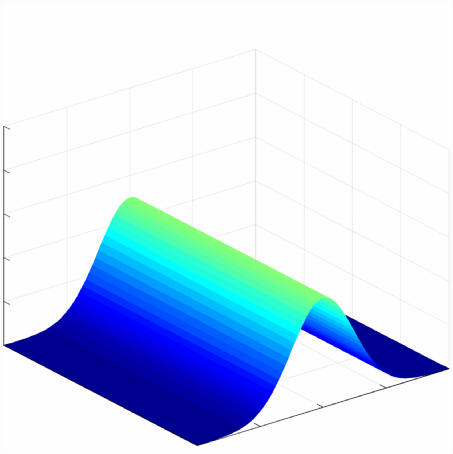
\includegraphics[width=0.2\textwidth]{\additivefigsdir/2d-kernel/additive_kernel_sum_p1} \hspace{-0.3cm}
& \hspace{-0.3cm} \raisebox{1cm}{$\times$} & 
\hspace{-0.3cm}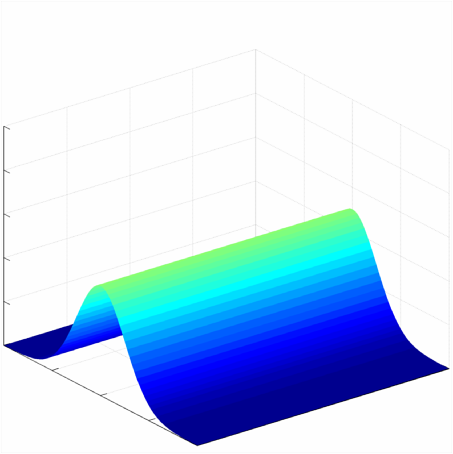
\includegraphics[width=0.2\textwidth]{\additivefigsdir/2d-kernel/additive_kernel_sum_p2} \hspace{-0.3cm}
& \hspace{-0.2cm} \raisebox{1cm}{=} \hspace{-0.2cm} & \hspace{-0.3cm}
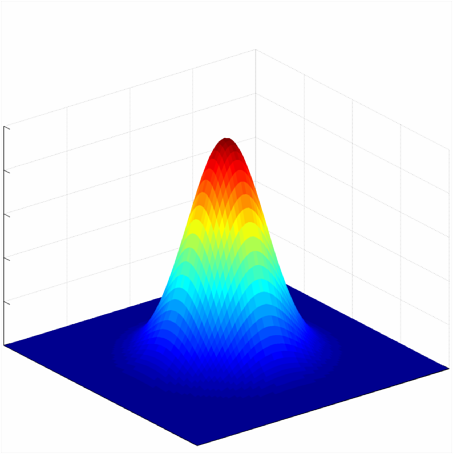
\includegraphics[width=0.2\textwidth]{\additivefigsdir/2d-kernel/sqexp_kernel} 
& \hspace{-0.3cm} \raisebox{1cm}{$\rightarrow$} \hspace{-0.3cm} & \hspace{-0.3cm}
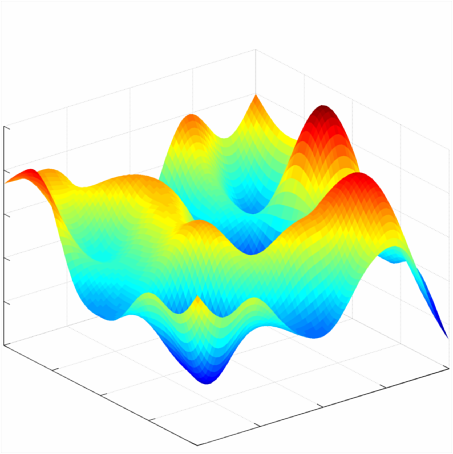
\includegraphics[width=0.2\textwidth]{\additivefigsdir/2d-kernel/sqexp_draw}\\
%$k_1(x_1, x_1')$ & & $k_2(x_2, x_2')$ & & \hspace{-0.4cm}\parbox{4cm}{$k_1(x_1,x_1') \kerntimes k_2(x_2,x_2')$} & & $f(x_1, x_2)$ \\[1em]
$\kSE_1(x_1, x_1')$ &  & $\kSE_2(x_2, x_2')$ &  & \hspace{-0.4cm} $\kSE_1 \kerntimes \kSE_2$ & & \hspace{-0.5cm} \parbox{0.24\columnwidth}{$f(x_1, x_2)$ drawn from $\GPt{0}{\kSE_1 \kerntimes \kSE_2}$} \\
\end{tabular}
\caption[A product of squared-exponential kernels across different dimensions]{
%\emph{Top left:} An additive kernel is a sum of kernels.
%\emph{Bottom left:}  A draw from an additive kernel corresponds to a sum of draws from independent \gp{} priors with the corresponding kernels.
%\emph{Top right:} A product kernel.
%\emph{Right:}  A \gp{} prior with a product of kernels does not correspond to a product of draws from \gp{}s.
%In this example, both kernels are composed of one dimensional squared-exponential kernels, but this need not be the case in general.
A product of two one-dimensional kernels gives rise to a prior on functions which depend on both dimensions.
}
\label{fig:product-of-se-kernels}
\end{figure}

\ARD{} stands for automatic relevance determination, so named because estimating the lengthscale parameters $\ell_1, \ell_2, \dots, \ell_D$, implicitly determines the ``relevance'' of each dimension.
Input dimensions with relatively large lengthscales imply relatively little variation along those dimensions in the function being modeled.

$\seard$ kernels are the default kernel in most applications of \gp{}s.
This may be partly because they have relatively few parameters to estimate, and because those parameters are relatively interpretable.
In addition, there is a theoretical reason to use them: they are \emph{universal} kernels~\citep{micchelli2006universal}, capable of learning any continuous function given enough data, under some conditions.

However, this flexibility means that they can sometimes be relatively slow to learn, due to the \emph{curse of dimensionality} \citep{bellman1956dynamic}.
In general, the more structure we account for, the less data we need - the \emph{blessing of abstraction} \citep{goodman2011learning} counters the curse of dimensionality.
Below, we will investigate ways to encode more structure into kernels.



\section{Modeling sums of functions}
\label{sec:modeling-sums-of-functions}
An additive function is one which can be expressed as $f(\vx) = f_a(\vx) + f_b(\vx)$.
Additivity is a useful modeling assumption in a wide variety of contexts, especially if it allows us to make strong assumptions about the individual components which make up the sum.
Restricting the flexibility of component functions often aids in building interpretable models, and sometimes enables extrapolation in high dimensions.

%TODO: make the se_long + se_short figure a bit more obvious
\begin{figure}[h]
\centering
\begin{tabular}{cccc}
%Composite & Draws from \gp{} & \gp{} posterior \\ \toprule
$\kLin + \kPer$ & $\kSE + \kPer$ & $\kSE + \kLin$ & $\kSE^{(\textnormal{long})} + \kSE^{(\textnormal{short})}$ \\
\kernpic{lin_plus_per} & \kernpic{se_plus_per} & \kernpic{se_plus_lin} & \kernpic{shortse_plus_medse}\\
\fixedx & $x -x'$ & \fixedx & $x -x'$\\
%& & & \\
\large $\downarrow$ & \large $\downarrow$ & \large $\downarrow$ & \large $\downarrow$  \\
\kernpic{lin_plus_per_draws} & \kernpic{se_plus_per_draws_s7} & \kernpic{se_plus_lin_draws_s5} & \kernpic{shortse_plus_medse_draws_s5}\\
periodic plus trend & periodic plus noise & linear plus variation & slow \& fast variation \\[10pt]
\end{tabular}
\caption[Examples of structures expressible by adding kernels]
{ Examples of one-dimensional structures expressible by adding kernels.  
%The x-axis has the same scale for all plots.
Rows have the same meaning as in \cref{fig:basic_kernels}.
$\kSE^{(\textnormal{long})}$ denotes a $\kSE$ kernel whose lengthscale is long relative to that of $\kSE^{(\textnormal{short})}$
}
\label{fig:kernels_plus}
\end{figure}

It is easy to encode additivity into \gp{} models.
Suppose functions ${\function_a, \function_b}$ are drawn independently from \gp{} priors:
%
\begin{align}
\function_a & \dist \GP(\mu_a, \kernel_a) \\
\function_b & \dist \GP(\mu_b, \kernel_b)
\end{align}
%
Then the distribution of the sum of those functions is simply another \gp{}:
%
\begin{align}
%\function := 
\function_a + \function_b \dist \GP(\mu_a + \mu_b, \kernel_a + \kernel_b).
\end{align}
%
Kernels $\kernel_a$ and $\kernel_b$ can be of different types, allowing us to model the data as a sum of independent functions, each possibly representing a different type of structure.
Any number of components can be summed this way.


\subsection{Modeling noise}

%We sometimes refer to a part of the signal that we don't care about, or don't expect to be able to extrapolate, as the noise.

Additive noise can be modeled as an unknown, quickly-varying function added to the signal.
This structure can be incorporated into a \gp{} model by adding a local kernel such as an \kSE{} with a short lengthscale, as in the fourth column of \cref{fig:kernels_plus}.
The limit of the $\kSE$ kernel as its lengthscale goes to zero is a ``white noise'' (\kWN) kernel.
Function values drawn from a \gp{} with a $\kWN$ kernel are independent draws from a Gaussian random variable.

Given a kernel containing both signal and noise components, we may wish to isolate only the signal components.
\Cref{sec:posterior-variance} shows how to decompose a \gp{} posterior into each of its additive components.

In practice, there may not be a clear distinction between signal and noise.
For example, \cref{sec:time_series} contains examples of models having long-term, medium-term, and short-term trends.
Which parts we designate as the ``signal'' sometimes depends on the task at hand.


\subsection{Additivity across multiple dimensions}
\label{sec:additivity-multiple-dimensions}

When modeling functions of multiple dimensions, summing kernels can give rise to additive structure across different dimensions.
To be more precise, if the kernels being added together are each functions of only a subset of input dimensions, then the implied prior over functions decomposes in the same way.
%
\begin{figure}
\centering
\begin{tabular}{ccccc}
\hspace{-0.2cm}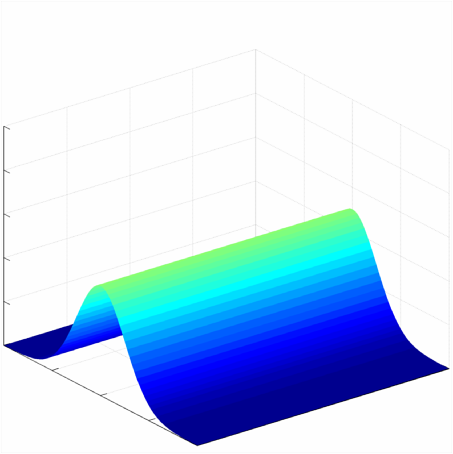
\includegraphics[width=0.2\textwidth]{\additivefigsdir/2d-kernel/additive_kernel_sum_p2} 
& \hspace{-0.4cm} \raisebox{1cm}{+} \hspace{-0.4cm} & 
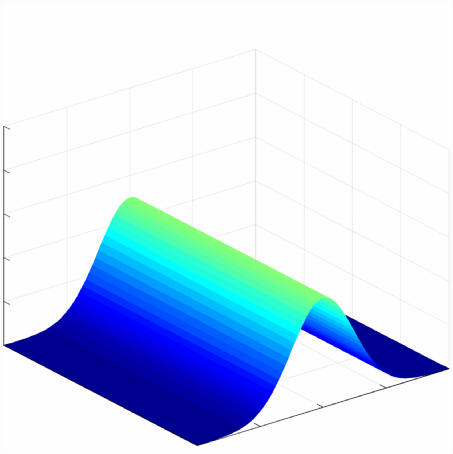
\includegraphics[width=0.2\textwidth]{\additivefigsdir/2d-kernel/additive_kernel_sum_p1} 
& \hspace{-0.4cm} \raisebox{1cm}{=} \hspace{-0.4cm} & 
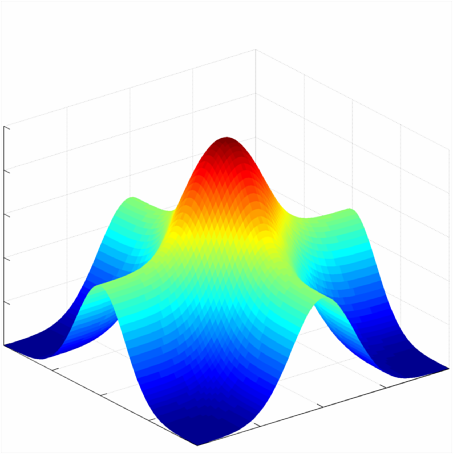
\includegraphics[width=0.2\textwidth]{\additivefigsdir/2d-kernel/additive_kernel} \\
$k_1(x_1, x_1')$ & & $k_2(x_2, x_2')$ & & $k_1(x_1,x_1') + k_2(x_2,x_2')$ \\[1em]
\large $\downarrow$ & & \large $\downarrow$ & & \large $\downarrow$ \\[-0.2em]
\hspace{-0.2cm}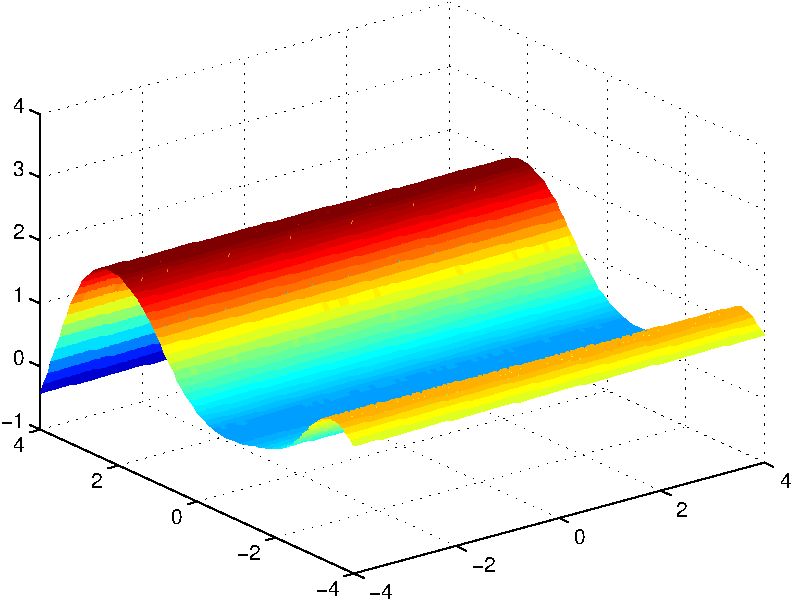
\includegraphics[width=0.2\textwidth]{\additivefigsdir/2d-kernel/additive_kernel_draw_sum_p1}
& \hspace{-0.4cm} \raisebox{1cm}{+} \hspace{-0.4cm} & 
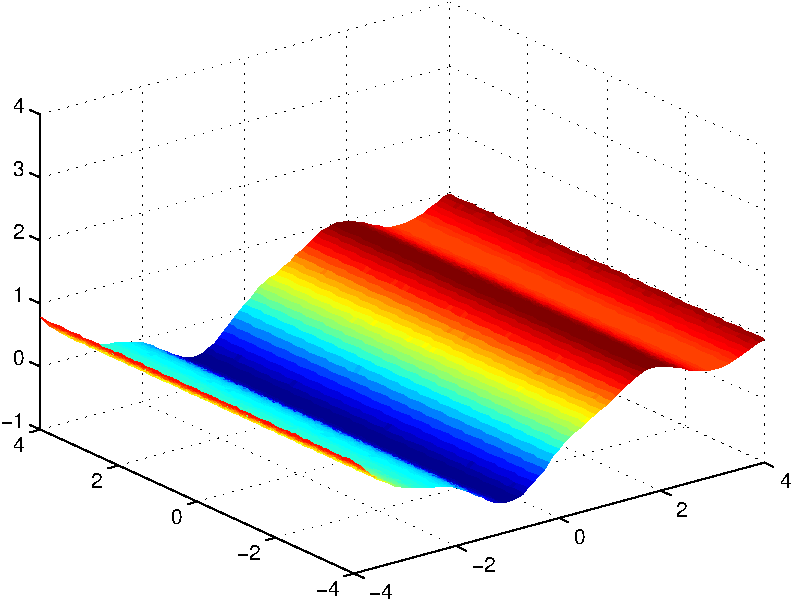
\includegraphics[width=0.2\textwidth]{\additivefigsdir/2d-kernel/additive_kernel_draw_sum_p2}
& \hspace{-0.4cm} \raisebox{1cm}{=} \hspace{-0.4cm} &
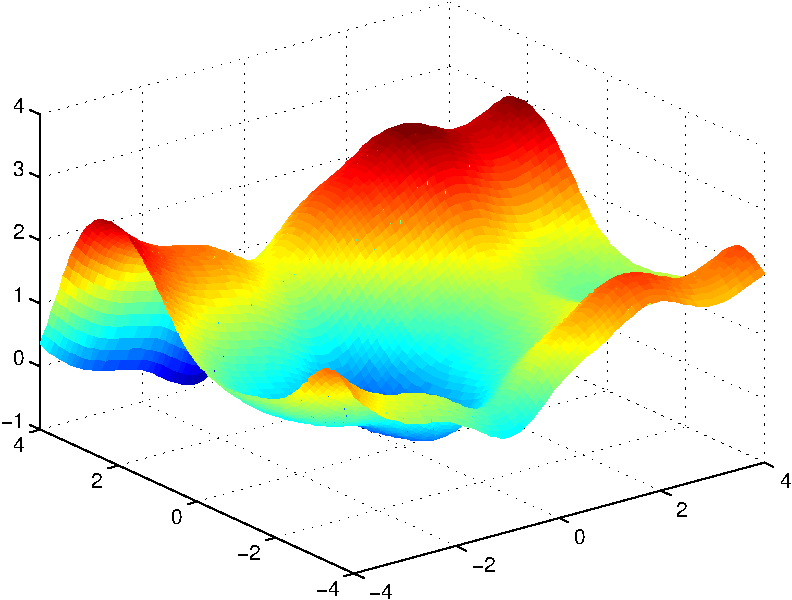
\includegraphics[width=0.2\textwidth]{\additivefigsdir/2d-kernel/additive_kernel_draw_sum} \\
$f_1(x_1) \sim \GP\left(0, k_1\right)$ & & $f_2(x_2) \sim \GP\left(0, k_2\right)$ & & $f_1(x_1) + f_2(x_2)$ \\[1em]
\end{tabular}
\caption[Additive kernels correspond to additive functions]{
A sum of two orthogonal one-dimensional kernels.
\emph{Top row:} An additive kernel is a sum of kernels.
\emph{Bottom row:} A draw from an additive kernel corresponds to a sum of draws from independent \gp{} priors, each having the corresponding kernel.
}
\label{fig:sum-of-kernels}
\end{figure}
%
For example,
%
\begin{align}
%\function := 
f(x_1, x_2) \dist \GP(0, \kernel_1(x_1, x_1') + \kernel_2(x_2, x_2'))
\label{eq:simple-additive-gp}
\end{align}
%
is equivalent to the model
%
\begin{align}
\function_1(x_1) & \dist \GP(0, \kernel_1(x_1, x_1'))\\
\function_2(x_2) & \dist \GP(0, \kernel_2(x_2, x_2'))\\
f(x_1, x_2) & = f_1(x_1) + f_2(x_2) \, .
\end{align}
%
%Then we can model the sum of those functions through another \gp{}:
%

\Cref{fig:sum-of-kernels} illustrates a decomposition of this form.
Note that the product of two kernels does not have an analogous interpretation as the product of two functions.


\subsection{Extrapolation through additivity}
\label{sec:additivity-extrapolation}

Additive structure sometimes allows us to make predictions far from the training data.
%
\begin{figure}
\centering
\begin{tabular}{ccc}
 & \gp{} mean using & \gp{} mean using \\
True function: & sum of $\kSE$ kernels: & product of $\kSE$ kernels: \\
\parbox{0.33\columnwidth}{$f(x_1, x_2) = \sin(x_1) + \sin(x_2)$} & $k_1(x_1, x_1') \kernplus k_2(x_2, x_2')$ &  $k_1(x_1, x_1') \kerntimes k_2(x_2, x_2')$ \\[0.2em]
\hspace{-0.1in}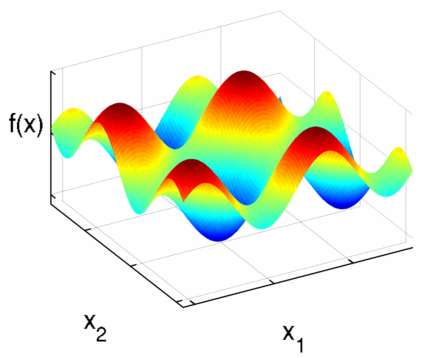
\includegraphics[width=0.32\textwidth]{\additivefigsdir/1st_order_censored_truth} &
\hspace{-0.1in}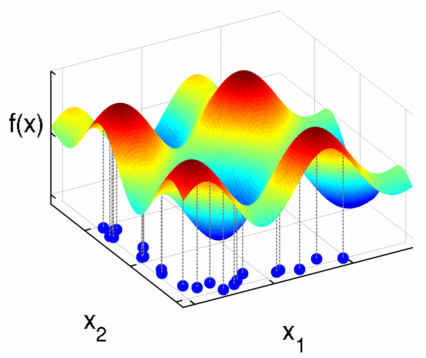
\includegraphics[width=0.32\textwidth]{\additivefigsdir/1st_order_censored_add} & 
\hspace{-0.1in}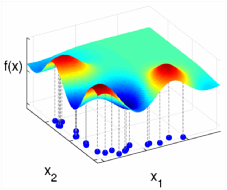
\includegraphics[width=0.32\textwidth]{\additivefigsdir/1st_order_censored_ard}\\[0em]
%,clip,trim=16mm 17mm 0mm 0mm
\end{tabular}
\caption[Extrapolation in functions with additive structure]
{\emph{Left:} A function with additive structure.
%Inference in functions with additive structure.
\emph{Center:} A \gp{} with an additive kernel can extrapolate away from the training data.
\emph{Right:} A \gp{} with a product kernel allows a different function value for every combination of inputs, and so is uncertain about function values away from the training data.  This causes the predictions to revert to the mean.
%  The additive GP is able to discover the additive pattern, and use it to fill in a distant mode.  The ARD kernel can only interpolate, and thus predicts the mean in locations missing data.
}
\label{fig:synth2d}
\end{figure}
%
\Cref{fig:synth2d} compares the extrapolations made by additive versus product-kernel \gp{} models, conditioned on data from a sum of two axis-aligned sine functions.
The training points were evaluated in a small, L-shaped area.
In this example, the additive model is able to correctly predict the height of the function at an unseen combinations of inputs.
The product-kernel model is more flexible, and so remains uncertain about the function away from the data.
%The ability of additive GPs to discover long-range structure suggests that this model may be well-suited to deal with covariate-shift problems.

These types of additive models have been well-explored in the statistics literature.
For example, generalized additive models~\citep{hastie1990generalized} have seen wide adoption.
In high dimensions, we can also consider sums of functions of multiple input dimensions.
\Cref{ch:additive} considers this model class in more detail.




\subsection{Example: An additive model of concrete strength}
\label{sec:concrete}

To illustrate how additive kernels give rise to interpretable models, we built an additive model of the strength of concrete as a function of the amount of seven different ingredients (cement, slag, fly ash, water, plasticizer, coarse aggregate and fine aggregate), and the age of the concrete \citep{yeh1998modeling}.
%We model measurements of the compressive strength of concrete, as a function of the concentration of 7 ingredients, plus the age of the concrete.
Our simple model is a sum of 8 different one-dimensional functions, each depending on one of these variables:
%
\begin{align}
f(\vx) & = 
f_1(\textnormal{cement}) + f_2(\textnormal{slag}) + f_3(\textnormal{fly ash}) + f_4(\textnormal{water}) \nonumber \\
& \quad + f_5(\textnormal{plasticizer}) + f_6(\textnormal{coarse}) + f_7(\textnormal{fine}) + f_8(\textnormal{age}) + \textnormal{noise}
\label{eq:concrete}
\end{align}
%
where $\textnormal{noise} \simiid \Nt{0}{\sigma^2_n}$.
%The corresponding kernel has 9 additive components.
Each of the functions $f_1, f_2, \ldots, f_8$ was modeled using a \gp{} with an $\kSE$ kernel.
These eight $\kSE$ kernels plus a white noise kernel were added together as in \cref{eq:simple-additive-gp} to form a single \gp{} model whose kernel had 9 additive components.

After learning the kernel parameters by maximizing the marginal likelihood of the data, one can visualize the predictive distribution of each component of the model.

\newcommand{\concretepic}[1]{\includegraphics[width=0.3\columnwidth]{\decompfigsdir/concrete-component-#1}}
\newcommand{\concretelegend}[0]{\raisebox{5mm}{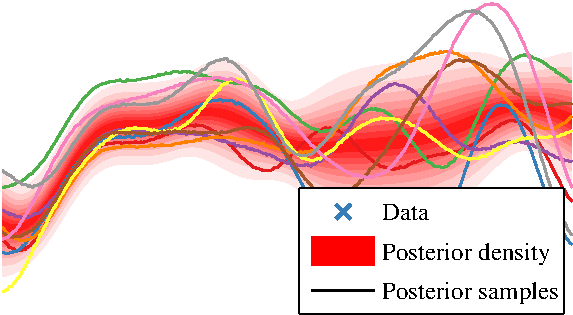
\includegraphics[trim=56mm 1mm 2.1mm 34mm, clip, width=0.24\columnwidth]{\decompfigsdir/concrete-component-8-legend}}}
%
\begin{figure}[h!]
\centering
\begin{tabular}{cccc}
%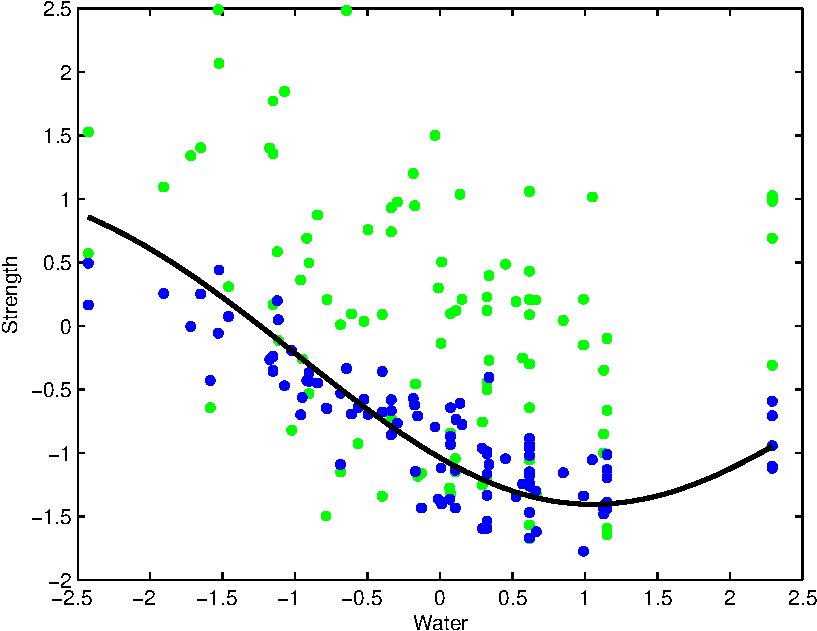
\includegraphics[width=0.3\textwidth]{\additivefigsdir/interpretable_1st_order1.pdf} &
%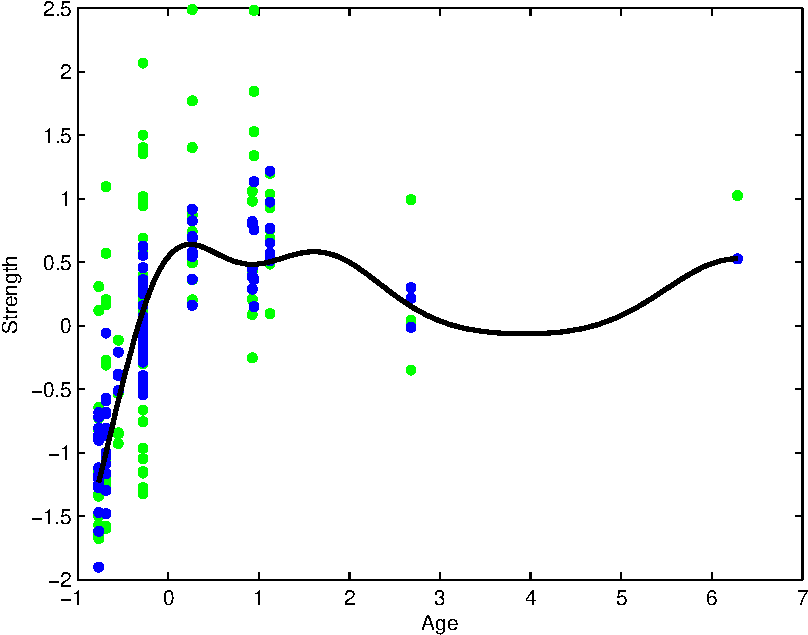
\includegraphics[width=0.3\textwidth]{\additivefigsdir/interpretable_1st_order2.pdf}& 
\hspace{-6mm}\raisebox{0.7cm}{\rotatebox{90}{strength}}\hspace{-7mm} &
\concretepic{1} & \concretepic{2} & \concretepic{3} \\
& cement (kg/m$^3$) & slag (kg/m$^3$) & fly ash (kg/m$^3$)\\[4mm]
\hspace{-6mm}\raisebox{0.7cm}{\rotatebox{90}{strength}}\hspace{-7mm} &
\concretepic{4} & \concretepic{5} & \concretepic{6} \\
& water (kg/m$^3$) & plasticizer (kg/m$^3$) & coarse (kg/m$^3$) \\[4mm]
\hspace{-6mm}\raisebox{0.7cm}{\rotatebox{90}{strength}}\hspace{-7mm} &
\concretepic{7} & \concretepic{8} & \concretelegend \\
& fine (kg/m$^3$) & age (days) \\
\end{tabular}
\caption[Decomposition of posterior into interpretable one-dimensional functions]
{The predictive distribution of each one-dimensional function in a multi-dimensional additive model.
Blue crosses indicate the original data projected on to each dimension, red indicates the marginal posterior density of each function, and colored lines are samples from the marginal posterior distribution of each one-dimensional function.
The vertical axis is the same for all plots.
%The black line is the posterior mean of a \sgp{} with only one term in its kernel.
%Right:  the posterior mean of a \sgp{} with only one second-order term in its kernel.
%rs = 1 - var(complete_mean - y)/ var(y)
%R-squared = 0.9094
}
\label{fig:interpretable functions}
\end{figure}

\Cref{fig:interpretable functions} shows the marginal posterior distribution of each of the eight one-dimensional functions in the model. %\cref{eq:concrete}.
The parameters controlling the variance of two of the functions, $f_6(\textnormal{coarse})$ and $f_7(\textnormal{fine})$ were set to zero, meaning that the marginal likelihood preferred a parsimonious model which did not depend on these inputs.
This is an example of the automatic sparsity that arises by maximizing marginal likelihood in \gp{} models, and another example of automatic relevance determination (\ARD) \citep{neal1995bayesian}.

The ability to learn kernel parameters in this way is much more difficult when using non-probabilistic methods such as Support Vector Machines \citep{cortes1995support}, for which cross-validation is often the best method to select kernel parameters.



\subsection{Posterior variance of additive components}
\label{sec:posterior-variance}


%\footnote{Code is available at \url{github.com/duvenaud/phd-thesis/}}
Here we derive the posterior variance and covariance of all of the additive components of a \gp{}.
These formulas allow one to make plots such as \cref{fig:interpretable functions}.
%These formulas let us plot the marginal variance of each component separately.  These formulas can also be used to examine the posterior covariance between pairs of components.

First, we write down the joint prior distribution over two functions drawn independently from \gp{} priors, and their sum.
We distinguish between $\vecf(\vX)$ (the function values at training locations $[\vx_1, \vx_2, \ldots, \vx_N]\tra \defeq \vX$) and  $\vecf(\vX^\star)$ (the function values at some set of query locations $[\vx_1^\star, \vx_2^\star, \ldots, \vx_N^\star]\tra \defeq \vX^\star$).
% so that it's clear which matrices to use to extrapolate.

Formally, if $f_1$ and $f_2$ are \emph{a priori} independent, and $f_1 \sim \gp( \mu_1, k_1)$ and ${f_2 \sim \gp( \mu_2, k_2)}$, then
%
\begin{align}
\left[ \! \begin{array}{l} 
\vf_1(\vX) \\
\vf_1(\vX^\star) \\
\vf_2(\vX) \\
\vf_2(\vX^\star) \\
\vf_1(\vX) + \vf_2(\vX) \\
\vf_1(\vX^\star) + \vf_2(\vX^\star)
\end{array} \! \right]
\sim
\Nt{
\left[ \! \begin{array}{c} \vmu_1 \\ \vmu_1^\star \\ \vmu_2 \\ \vmu_2^\star \\ \vmu_1 + \vmu_2 \\ \vmu_1^\star + \vmu_2^\star \end{array} \! \right] \!
}
{\! \left[ \! \begin{array}{llllll}%{cccccc} 
\vK_1 & \vK_1^\star & 0 & 0 & \vK_1 & \vK_1^\star \\ 
{\vK_1^\star}\tra & \vK_1^{\star\star} & 0 & 0 & \vK_1^\star & \vK_1^{\star\star} \\
0 & 0 & \vK_2 & {\vK_2^\star} & \vK_2 & \vK_2^\star \\ 
0 & 0 & {\vK_2^\star}\tra & \vK_2^{\star\star} & \vK_2^\star & \vK_2^{\star\star} \\
{\vK_1} & {\vK_1^\star}\tra & \vK_2 & {\vK_2^\star}\tra & \vK_1 + \vK_2 & \vK_1^\star + \vK_2^\star \\ 
{\vK_1^\star}\tra & \vK_1^{\star\star}  & {\vK_2^\star}\tra & \vK_2^{\star\star}  & {\vK_1^\star}\tra + {\vK_2^\star}\tra & \vK_1^{\star\star} + \vK_2^{\star\star}\\
\end{array} \! \right]
}
\end{align}
%
where we represent the Gram matrices, whose $i,j$th entry is given by $k(\vx_i, \vx_j)$ by
% evaluated at all pairs of vectors in bold capitals as ${\vK_{i,j} = k(\vx_i, \vx_j)}$.
%
\begin{align}
\vK_i & = k_i( \vX, \vX ) \\
\vK_i^\star & = k_i( \vX, \vX^\star ) \\
\vK_i^{\star\star} & = k_i( \vX^\star, \vX^\star )
\end{align}

The formula for Gaussian conditionals \ref{eq:gauss_conditional} can be used to give the conditional distribution of a \gp{}-distributed function conditioned on its sum with another \gp{}-distributed function:
%
\begin{align}
\vf_1(\vX^\star) \big| \vf_1(\vX) + \vf_2(\vX) \sim \Normal \Big( 
& \vmu_1^\star + \vK_1^{\star\tra} (\vK_1 + \vK_2)\inv \big[ \vf_1(\vX) + \vf_2(\vX) - \vmu_1 - \vmu_2 \big], \nonumber \\
& \vK_1^{\star\star} - \vK_1^{\star\tra} (\vK_1 + \vK_2)\inv \vK_1^{\star} \Big)
%\vf_1(\vx^\star) | \vf(\vx) \sim \mathcal{N}\big( 
%& \vmu_1(\vx^\star) + \vk_1(\vx^{\star}, \vx)  \left[ \vK_1(\vx, \vx) + \vK_2(\vx, \vx) \right]\inv \left( \vf(\vx) - \vmu_1(\vx) - \vmu_2(\vx) \right) , \nonumber \\
%& \vk_1(\vx^{\star}, \vx^{\star}) - \vk_1(\vx^{\star}, \vx)  \left[ \vK_1(\vx, \vx) + \vK_2(\vx, \vx) \right] \inv \vk_1(\vx, \vx^{\star}) 
%\big).
\end{align}
%
These formulas express the model's posterior uncertainty about the different components of the signal, integrating over the possible configurations of the other components.
To extend these formulas to a sum of more than two functions, the term $\vK_1 + \vK_2$ can simply be replaced by $\sum_i \vK_i$ everywhere.




\subsubsection{Posterior covariance of additive components}

%One of the advantages of using a generative, model-based approach is that we can examine any aspect of the model we wish to.
One can also compute the posterior covariance between the height of any two functions, conditioned on their sum:
%
\begin{align}
\Cov \big[ \vf_1(\vX^\star), \vf_2(\vX^\star) \big| \vf(\vX) \big]
& = - \vK_1^{\star\tra} (\vK_1 + \vK_2)\inv \vK_2^\star
%\covargs{\vf_1(\vx^\star)}{\vf_2(\vx^\star) | \vf(\vx) }
%& = - \vk_1(\vx^{\star}, \vx)  \left[ \vK_1(\vx, \vx) + \vK_2(\vx, \vx) \right] \inv \vk_1(\vx, \vx^{\star}) 
\label{eq:post-component-cov}
\end{align}
%
If this quantity is negative, it means that there is ambiguity about which of the two functions is high or low at that location.
\begin{figure}
\centering
\renewcommand{\tabcolsep}{1mm}
\def\incpic#1{\includegraphics[width=0.11\columnwidth]{../figures/decomp/concrete-#1}}
\begin{tabular}{p{2mm}*{6}{c}}
  & {cement} & {slag} & {fly ash} & {water} & \parbox{0.1\columnwidth}{plasticizer} & {age} \\
 \rotatebox{90}{{$\;\;$cement}} & \incpic{Cement-Cement} & \incpic{Cement-Slag} & \incpic{Cement-Fly-Ash} & \incpic{Cement-Water} & \incpic{Cement-Plasticizer} & \incpic{Cement-Age} \\ 
 \rotatebox{90}{{$\;\;$$\;\;$slag}} & \incpic{Slag-Cement} & \incpic{Slag-Slag} & \incpic{Slag-Fly-Ash} & \incpic{Slag-Water} & \incpic{Slag-Plasticizer} & \incpic{Slag-Age} \\ 
 \rotatebox{90}{{$\;\;$fly ash}} & \incpic{Fly-Ash-Cement} & \incpic{Fly-Ash-Slag} & \incpic{Fly-Ash-Fly-Ash} & \incpic{Fly-Ash-Water} & \incpic{Fly-Ash-Plasticizer} & \incpic{Fly-Ash-Age} \\ 
 \rotatebox{90}{{$\quad$water}} & \incpic{Water-Cement} & \incpic{Water-Slag} & \incpic{Water-Fly-Ash} & \incpic{Water-Water} & \incpic{Water-Plasticizer} & \incpic{Water-Age} \\ 
 \rotatebox{90}{{plasticizer}} & \incpic{Plasticizer-Cement} & \incpic{Plasticizer-Slag} & \incpic{Plasticizer-Fly-Ash} & \incpic{Plasticizer-Water} & \incpic{Plasticizer-Plasticizer} & \incpic{Plasticizer-Age}\\
\rotatebox{90}{$\;\;$$\;\;$\phantom{t}age} & \incpic{Age-Cement} & \incpic{Age-Slag} & \incpic{Age-Fly-Ash} & \incpic{Age-Water} & \incpic{Age-Plasticizer} & \incpic{Age-Age} \\
 \end{tabular}
 \fbox{
\begin{tabular}{c}
 Correlation \\[1ex]
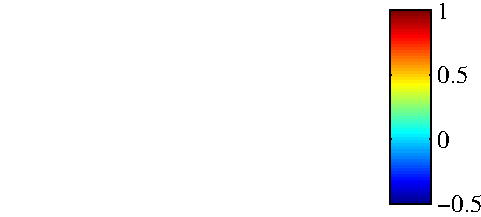
\includegraphics[width=0.1\columnwidth, clip, trim=6.2cm 0cm 0cm 0cm]{../figures/decomp/concrete-colorbar}
\end{tabular}
}
\caption[Visualizing posterior correlations between components]
{Posterior correlations between the heights of the one-dimensional functions in \cref{eq:concrete}, whose sum models concrete strength.
%Each plot shows the posterior correlations between the height of two functions, evaluated across the range of the data upon which they depend.
%Color indicates the amount of correlation between the function value of the two components.
Red indicates high correlation, teal indicates no correlation, and blue indicates negative correlation.
Plots on the diagonal show posterior correlations within each function.
Correlations are evaluated over the same input ranges as in \cref{fig:interpretable functions}. 
%Off-diagonal plots show posterior covariance between each pair of functions, as a function of both inputs.
%Negative correlation means that one function is high and the other low, but which one is uncertain.
Correlations with $f_6(\textnormal{coarse})$ and $f_7(\textnormal{fine})$ are not shown, because their estimated variance was zero.
}
\label{fig:interpretable interactions}
\end{figure}
%
For example, \cref{fig:interpretable interactions} shows the posterior correlation between all non-zero components of the concrete model.
This figure shows that most of the correlation occurs within components, but there is also negative correlation between the ``cement'' and ``slag'' variables.
This reflects an ambiguity in the model about which one of these functions is high and the other low.






\section{Changepoints}
\label{sec:changepoint-definition}
An example of how combining kernels can give rise to more structured priors is given by changepoint kernels, which can express a change between different types of structure.
Changepoints kernels can be defined through addition and multiplication with sigmoidal functions such as $\sigma(x) = \nicefrac{1}{1 + \exp(-x)}$:
%
\begin{align}
%\kCP(\kernel_1, \kernel_2) = \kernel_1 \kerntimes \boldsymbol\sigma \kernplus \kernel_2 \kerntimes \boldsymbol{\bar\sigma}
%\kCP(\kernel_1, \kernel_2) & = \begin{array}{rl} (1-\sigma(x)) & k_2(x,x')(1-\sigma(x')) \\
%  + \sigma(x) & k_1(x,x')\sigma(x') \end{array} \\
\kCP(\kernel_1, \kernel_2)(x,x') & = \sigma(x) k_1(x,x')\sigma(x') + (1-\sigma(x)) k_2(x,x')(1-\sigma(x'))
\label{eq:cp}
\end{align}
%
which can be written in shorthand as
%
\begin{align}
\kCP(\kernel_1, \kernel_2)& = \kernel_1 \kerntimes \boldsymbol\sigma \kernplus \kernel_2 \kerntimes \boldsymbol{\bar\sigma}
\end{align}
where $\boldsymbol\sigma = \sigma(x)\sigma(x')$ and $\boldsymbol{\bar\sigma} = (1-\sigma(x))(1-\sigma(x'))$.

This compound kernel expresses a change from one kernel to another.
The parameters of the sigmoid determine where, and how rapidly, this change occurs.
Figure~\ref{fig:changepoint_examples} shows some examples.
%
\newcommand{\cppic}[1]{\includegraphics[height=2.2cm,width=3.3cm]{\grammarfiguresdir/changepoint/#1}}%
\begin{figure}[h]
\centering
\begin{tabular}{rcccc}
 & $\kCP(\kSE, \kPer)$ & $\kCP(\kSE, \kPer)$ & $\kCP(\kSE, \kSE)$ & $\kCP(\kPer, \kPer)$ \\
\raisebox{1cm}{$f(x)$} \hspace{-0.4cm} & \cppic{draw_1} & \cppic{draw_2} & \cppic{draw_3} & \cppic{draw_4} \\
& $x$ & $x$ & $x$ & $x$
\end{tabular}
\caption[Draws from changepoint priors]
{Draws from different priors on using changepoint kernels, constructed by adding and multiplying together base kernels with sigmoidal functions.
}
\label{fig:changepoint_examples}
\end{figure}

We can also build a model of functions whose structure changes only within some interval -- a \emph{change-window} -- by replacing $\sigma(x)$ with a product of two sigmoids, one increasing and one decreasing.

\subsection{Multiplication by a known function}

More generally, we can model an unknown function that's been multiplied by any fixed, known function $a(x)$, by multiplying the kernel by $a(\vx) a(\vx')$.
Formally,
%
\begin{align}
f(\iva) = a(\iva) g(\iva), \quad g \sim \GPdisttwo{0}{k(\iva, \iva')} \quad
\iff
\quad f \sim \GPdisttwo{0}{ a(\iva) k(\iva, \iva') a(\iva')} .
\end{align}




\section{Feature representation of kernels}
\label{sec:mercer}
%
By Mercer's theorem \citep{mercer1909functions},
%Due to \citet{mercer1909functions}, we know that
any positive-definite kernel can be represented as the inner product between a fixed set of features, evaluated at $\vx$ and at $\vx'$:
%
\begin{align}
k(\vx, \vx') = \feat(\vx)\tra \feat(\vx')
\end{align}

For example, the squared-exponential kernel ($\kSE$) on the real line has a representation in terms of infinitely many radial-basis functions of the form ${h_i(x) \propto \exp( -\frac{1}{4\ell^2} (x - c_i)^2)}$.
More generally, any stationary kernel can be represented by a set of sines and cosines - a Fourier representation \citep{bochner1959lectures}.
In general, any particular feature representation of a kernel is not necessarily unique~\citep{minh2006mercer}.

In some cases, the input to a kernel, $\vx$, can even be the implicit infinite-dimensional feature mapping of another kernel.
Composing feature maps in this way leads to \emph{deep kernels}, which are explored in \cref{sec:deep_kernels}.
%\cref{ch:deep-limits}.



\subsection{Relation to linear regression}

Surprisingly, \gp{} regression is equivalent to Bayesian linear regression on the implicit features $\feat(\vx)$ which give rise to the kernel:
%
\begin{align}
f(\iva) = \vw\tra \feat(\iva), \quad \vw \sim \Nt{0}{\vI} \quad
\iff
\quad f \sim \GPdisttwo{0}{\feat(\iva) \tra \feat(\iva)}
\end{align}
%
The link between Gaussian processes, linear regression, and neural networks is explored further in \cref{sec:relating}.
%\cref{ch:deep-limits}.


\subsection{Feature-space view of combining kernels}

\def\feata{\va}
\def\featb{\vb}

%Many architectures for learning complex functions, such as convolutional networks \cite{lecun1989backpropagation} and sum-product networks \cite{poon2011sum}, include units which compute \texttt{and}-like and \texttt{or}-like operations.
%Composite kernels can be viewed in this way too.
%A sum of kernels can be understood as an \texttt{or}-like operation: two points are considered similar if either kernel has a high value.
%Similarly, multiplying kernels is an \texttt{and}-like operation, since two points are considered similar only if both kernels have high values.


We can also view kernel addition and multiplication as a combination of the features of the original kernels.
%Viewing kernel addition from this point of view, if
For example, given two kernels
%
\begin{align}
k_a(\iva, \iva') & = \feata(\iva)\tra \feata(\iva')\\
k_b(\iva, \iva') & = \featb(\iva)\tra \featb(\iva')
\end{align}
%
their addition has the form:
%
\begin{align}
k_a(\iva, \iva') + k_b(\iva, \iva')
& = \feata(\iva)\tra \feata(\iva') + \featb(\iva)\tra \featb(\iva') 
 = \colvec{\feata(\iva)}{\featb(\iva)}\tra \colvec{\feata(\iva')}{\featb(\iva')}
\end{align}
%
meaning that the features of $k_a + k_b$ are the concatenation of the features of each kernel.

We can examine kernel multiplication in a similar way:
%
\begin{align}
k_a(\iva, \iva') \times k_b(\iva, \iva')
& = \left[ \feata(\iva)\tra \feata(\iva') \right] \times \left[ \featb(\iva)\tra \featb(\iva') \right] \\
%& = \left[ \begin{array}{c} \feat_1(\iva) \\ \feat_2(\iva) \end{array} \right]^\tra \left[ \begin{array}{c} \feat_1(\iva') \\ \feat_2(\iva') \end{array} \right]
& = \sum_i a_i(\iva) a_i(\iva') \times \sum_j b_j(\iva) b_j(\iva') \\
%& = \sum_i \sum_j a_i(\iva) a_i(\iva') b_j(\iva) b_j(\iva') \\
& = \sum_{i,j} \big[ a_i(\iva) b_j(\iva) \big] \big[ a_i(\iva') b_j(\iva') \big]
%& = \vecop{ \feata(\iva) \otimes \featb(\iva') } \tra \vecop{ \feata(\iva) \otimes \featb(\iva')} 
\end{align}
%
In words, the features of $k_a \kerntimes k_b$ are made of up all pairs of the original two sets of features.
For example, the features of the product of two one-dimensional $\kSE$ kernels $(\kSE_1 \kerntimes \kSE_2)$ cover the plane with two-dimensional radial-basis functions of the form:
%
\begin{align}
h_{ij}(x_1, x_2) \propto \exp \left( -\frac{1}{2} \frac{(x_1 - c_i)^2}{2\ell_1^2} \right) \exp \left( -\frac{1}{2} \frac{(x_2 - c_j)^2}{2\ell_2^2} \right)
\end{align}





\section{Expressing symmetries and invariances}
\label{sec:expressing-symmetries}

\def\gswitch{G_\textnormal{swap}}

When modeling functions, encoding known symmetries can improve predictive accuracy. 
This section looks at different ways to encode symmetries into a prior on functions.
Many types of symmetry can be enforced through operations on the kernel.

We will demonstrate the properties of the resulting models by sampling functions from their priors.
By using these functions to define smooth mappings from $\Reals^2 \to \Reals^3$, we will show how to build a nonparametric prior on an open-ended family of topological manifolds, such as cylinders, toruses, and M\"{o}bius strips.

\subsection{Three recipes for invariant priors}

Consider the scenario where we have a finite set of transformations of the input space $\{g_1, g_2, \ldots \}$ to which we wish our function to remain invariant:
%
\begin{align}
f(\vx) = f(g(\vx))  \quad \forall \vx \in \mathcal{X}, \quad \forall g \in G
\end{align}
%
As an example, imagine we wish to build a model of functions invariant to swapping their inputs: $f(x_1, x_2) = f(x_2, x_1)$, $\forall x_1,x_2$.
Being invariant to a set of operations is equivalent to being invariant to all compositions of those operations, the set of which forms a group. \citep[chapter 21]{armstrong1988groups}.
In our example, the elements of the group $\gswitch$ containing all operations the functions are invariant to has two elements:%, and is an example of the symmetric group $S2$:
%
\begin{align}
g_1([x_1, x_2]) & = [x_2, x_1] \qquad \textnormal{(swap)} \\
g_2([x_1, x_2]) & = [x_1, x_2] \qquad \textnormal{(identity)}
\end{align}


How can we construct a prior on functions which respect these symmetries?
\citet{ginsbourger2012argumentwise} and \citet{Invariances13} showed that the only way to construct a \gp{} prior on functions which respect a set of invariances is to construct a kernel which respects the same invariances with respect to each of its two inputs:
%
\begin{align}
k(\vx, \vx') = k( g(\vx), g(\vx')), \quad \forall \vx, \vx' \in \InputSpace, \quad \forall g, g' \in G
\end{align}
%
Formally, given a finite group $G$ whose elements are operations to which we wish our function to remain invariant, and $f \sim \GPt{0}{k(\vx,\vx')}$, then every $f$ is invariant under $G$ (up to a modification) if and only if $k(\cdot, \cdot)$ is argument-wise invariant under $G$.
See \citet{Invariances13} for details.

It might not always be clear how to construct a kernel respecting such argument-wise invariances.
%Fortunately, for finite groups, there are a few simple ways to transform any kernel into one which is argument-wise invariant to actions under any finite group:
Fortunately, there are a few simple ways to do this for any finite group:
%
%
\begin{figure}
\renewcommand{\tabcolsep}{1.5mm}
\begin{tabular}{ccc}
Additive method & Projection method & Product method \\[0.5ex]
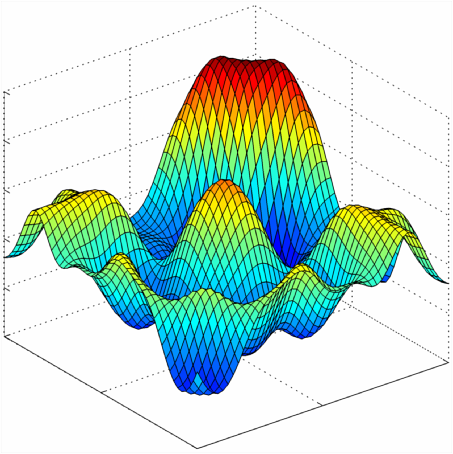
\includegraphics[width=0.3\columnwidth]{\symmetryfigsdir/symmetric-xy-naive-sample} &
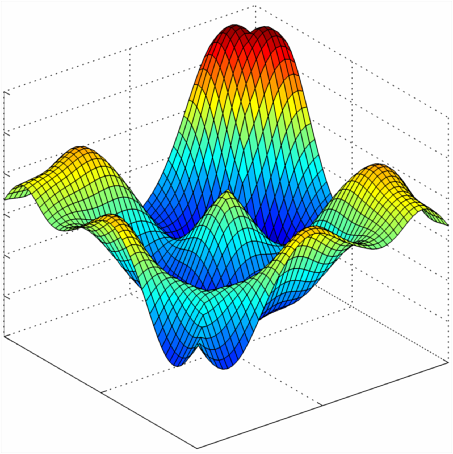
\includegraphics[width=0.3\columnwidth]{\symmetryfigsdir/symmetric-xy-projection-sample} &
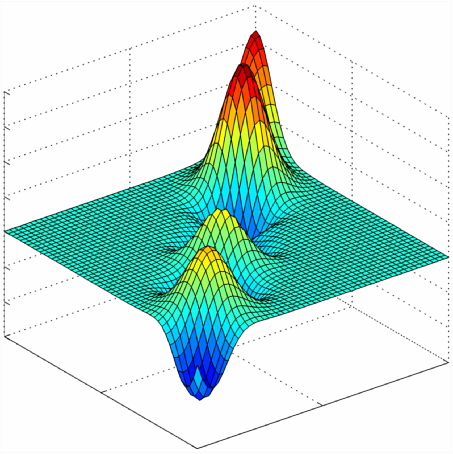
\includegraphics[width=0.3\columnwidth]{\symmetryfigsdir/symmetric-xy-prod-sample}\\
%$k(x, y, x', y') + k(x, y, y', x')$ & $k(x, y, x', y') \times k(x, y, y', x')$ & $k( \min(x, y), \max(x,y),$ \\
% $+ k(y, x, x', y') + k(y, x, y', x')$ & $\times k(y, x, x', y') \times k(y, x, y', x')$ & $\min(x', y'), \max(x',y') )$
%Draw from \gp{} with kernel: & Draw from \gp{} with kernel: &  Draw from \gp{} with kernel: \\
$\begin{array}{r@{}l@{}}
%& \kSE(x_1, x_2, x_1', x_2') \\ + \,\, & \kSE(x_1, x_2, x_2', x_1')
& \kSE(x_1, x_1')\kerntimes \kSE(x_2, x_2') \\ + \,\, & \kSE(x_1, x_2')\kerntimes\kSE(x_2, x_1')
\end{array}$
&
$\begin{array}{r@{}l@{}}
&            \kSE( \min(x_1, x_2),   \min(x_1', x_2')) \\
\kerntimes & \kSE( \max(x_1', x_2'), \max(x_1',x_2') )
\end{array}$
&
$\begin{array}{r@{}l@{}}
& \kSE(x_1, x_1')\kerntimes \kSE( x_2, x_2') \\ \times \,\, & \kSE(x_1, x_2')\kerntimes \kSE(x_2, x_1')
\end{array}$
\end{tabular}
\caption[Three ways to introduce symmetry]{
Functions drawn from three distinct \gp{} priors, each expressing symmetry about the line $x_1 = x_2$ using a different type of construction.
%Three methods of introducing symmetry, illustrated through draws from the corresponding priors.
%Left:  The additive method.
%Center: The product method.
%Right: The projection method.
%The additive method has half the marginal variance away from $y = x$, but the min method introduces a non-differentiable seam along $y = x$.
All three methods introduce a different type of nonstationarity.
}
\label{fig:add_vs_min}
\end{figure}
%
\begin{enumerate}

\item {\bf Sum over the orbit.} 
The \emph{orbit} of $x$ with respect to a group $G$ is ${\{g(x) : g \in G\}}$, the set obtained by applying each element of $G$ to $x$.
\citet{ginsbourger2012argumentwise} and \citet{kondor2008group} suggest enforcing invariances through a double sum over the orbits of $\vx$ and $\vx'$ with respect to G:
%
\begin{align}
k_\textnormal{sum}(\vx, \vx') = \sum_{g, \in G} \sum_{g' \in G} k( g( \vx ), g'( \vx') )
\end{align}

For the group $\gswitch$, this operation results in the kernel:
%
\begin{align}
k_\textnormal{switch}(\vx, \vx')
& = \sum_{g \in \gswitch} \sum_{g' \in \gswitch} k( g( \vx ), g'( \vx') ) \\
& = k(x_1, x_2, x_1', x_2') + k(x_1, x_2, x_2', x_1')  \nonumber \\ 
& \quad + k(x_2, x_1, x_1', x_2') + k(x_2, x_1, x_2', x_1')
\end{align}
%
For stationary kernels, some pairs of elements in this sum will be identical, and can be ignored.
\Cref{fig:add_vs_min}(left) shows a draw from a \gp{} prior with a product of $\kSE$ kernels symmetrized in this way.
This construction has the property that the marginal variance is doubled near $x_1 = x_2$, which may or may not be desirable.



\item {\bf Project onto a fundamental domain.}
\citet{Invariances13} also explored the possibility of projecting each datapoint into a fundamental domain of the group, using a mapping $A_G$:
%
\begin{align}
k_\textnormal{proj}(\vx, \vx') = k( A_G(\vx), A_G( \vx') )
\end{align}
%
For example, a fundamental domain of the group $\gswitch$ is all ${\{x_1, x_2 : x_1 < x_2\}}$, a set which can be mapped to using $A_{\gswitch}( x_1, x_2 ) = \big[ \min(x_1, x_2), \max(x_1, x_2) \big]$.
Constructing a kernel using this method introduces a non-differentiable  ``seam'' along $x_1 = x_2$, as shown in \cref{fig:add_vs_min}(center).
%The projection method also works for infinite groups, as we shall see below.

\item {\bf Multiply over the orbit.}
%\citet{adams2013product}
Ryan P. Adams (personal communication) suggested a construction enforcing invariances through a double product over the orbits:
%
\begin{align}
k_\textnormal{sum}(\vx, \vx') = \prod_{g \in G} \prod_{g' \in G} k( g( \vx ), g'( \vx') )
\end{align}
%
This method can sometimes produce \gp{} priors with zero variance in some regions, as in \cref{fig:add_vs_min}(right).
%We include it here to show that each of these methods for enforcing symmetries modifies the resulting model in other ways as well.
\end{enumerate}
%
There are often many possible ways to achieve a given symmetry, but we must be careful to do so without compromising other qualities of the model we are constructing.
For example, simply setting $k(\vx, \vx') = 0$ gives rise to a \gp{} prior which obeys \emph{all possible} symmetries, but this is presumably not a model we wish to use.




%In this section, we give recipes for expressing several classes of symmetries.  Later, we will show how these can be combined to produce more interesting structures.


\subsection{Example: Periodicity}

%We can enforce periodicity on any subset of the dimensions:
Periodicity in a one-dimensional function corresponds to the invariance
%
\begin{align}
f(x) = f( x + \tau)
\label{eq:periodic_invariance}
\end{align}
%
where $\tau$ is the period.

The most popular method for building a periodic kernel is due to \citet{mackay1998introduction}, who used the projection method in combination with an $\kSE$ kernel.
A fundamental domain of the symmetry group is a circle, so the kernel
%
%The representer transformation for periodicity is simply $A(x) = [\sin(x), \cos(x)]$:
%
\begin{align}
\kPer(x, x') = \kSE \left( \sin(x), \sin(x') \right) \kerntimes \kSE \left( \cos(x), \cos(x') \right)
\end{align}
%
%We can also apply rotational symmetry repeatedy to a single dimension.
achieves the invariance in \cref{eq:periodic_invariance}.
Simple algebra reduces this kernel to the form given in \cref{fig:basic_kernels}.

%We could also build a periodic kernel with period $\tau$ by the mapping $A(x) = \mod(x, \tau)$.
%However, samples from this prior would be discontinuous at every integer multiple of $\tau$.

\subsection{Example: Symmetry about zero}

Another example of an easily-enforceable symmetry is symmetry about zero:
%
\begin{align}
f(x) = f( -x) .
\end{align}
%
This symmetry can be enforced using the sum over orbits method, by the transform
%
\begin{align}
k_{\textnormal{reflect}}(x, x') & = k(x, x') + k(x, -x') + k(-x, x') + k(-x, -x').
\end{align}

%This transformation can be applied to any subset of dimensions

%\paragraph{Spherical Symmetry}

%We can also enforce that a function expresses the symmetries obeyed by $n-spheres$ by simply transforming a set of $n - 1$ coordinates by:
%
%\begin{align}
%x_1 & = \cos(\phi_1) \nonumber \\
%x_2 & = \sin(\phi_1) \cos(\phi_2) \nonumber \\
%x_3 & = \sin(\phi_1) \sin(\phi_2) \cos(\phi_3) \nonumber \\
%& \vdots \nonumber \\
%x_{n-1} & = \sin(\phi_1) \cdots \sin(\phi_{n-2}) \cos(\phi_{n-1}) \nonumber \\
%x_n & = \sin(\phi_1) \cdots \sin(\phi_{n-2}) \sin(\phi_{n-1})
%\end{align}

%\cite{flanders1989}



\subsection{Example: Translation invariance in images}

Many models of images are invariant to spatial translations \citep{lecun1995convolutional}.
Similarly, many models of sounds are also invariant to translation through time.

Note that this sort of translation invariance is completely distinct from the stationarity of kernels such as $\kSE$ or $\kPer$.
A stationary kernel implies that the prior is invariant to translations of the entire training and test set.
In contrast, here we use translation invariance to refer to situations where the signal has been discretized, and each pixel (or the audio equivalent) corresponds to a different input dimension.
We are interested in creating priors on functions that are invariant to swapping pixels in a manner that corresponds to shifting the signal in some direction:
%
\begin{align}
f \Bigg( \raisebox{-2.5ex}{ 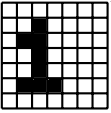
\includegraphics[width=1cm]{\topologyfiguresdir/grid2} } \Bigg) 
= f \Bigg( \raisebox{-2.5ex}{ 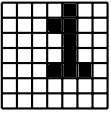
\includegraphics[width=1cm]{\topologyfiguresdir/grid3} } \Bigg)
\end{align}
%
%In this setting, translation is equivalent to swapping dimensions of the input vector $\vx$.
For example, in a one-dimensional image or audio signal, translation of an input vector by $i$ pixels can be defined as
%
\begin{align}
\shift(\vx, i) = \big[ x_{\mod( i + 1, D )}, x_{\mod( i + 2, D )}, \dots, x_{\mod( i + D, D )} \big]\tra
\end{align}
%
As above, translation invariance in one dimension can be achieved by a double sum over the orbit, given an initial translation-sensitive kernel between signals $k$:
%
\begin{align}
%k \left( (x_1, x_2, \dots, x_D ), (x_1', x_2', \dots, x_D' ) \right) & = %\nonumber \\
%\sum_{i=1}^D \prod_{j=1}^D k( x_j, x_{ i + j \textnormal{mod $D$} }' )
k_\textnormal{invariant} \left( \vx, \vx' \right) = %\nonumber \\
\sum_{i=1}^D \sum_{j=1}^D k( \shift(\vx, i), \shift(\vx, j) ) \,.
\end{align}
%
%This construction defines the kernel between two signals to be the sum of a kernel between all translations of those two signals.

The extension to two dimensions, $\shift(\vx, i, j)$, is straightforward, but notationally cumbersome.
\citet{kondor2008group} built a more elaborate kernel between images that was approximately invariant to both translation and rotation, using the projection method.

%Is there a pathology of the additive construction that appears in the limit?

%\subsection{Max-pooling}
%What we'd really like to do is a max-pooling operation.  However, in general, a kernel which is the max of other kernels is not PSD [put counterexample here?].  Is the max over co-ordinate switching PSD?





\section{Generating topological manifolds}
\label{sec:topological-manifolds}

In this section we give a geometric illustration of the symmetries encoded by different compositions of kernels.
The work presented in this section is based on a collaboration with David Reshef, Roger Grosse, Joshua B. Tenenbaum, and Zoubin Ghahramani.
The derivation of the M\"obius kernel was my original contribution.

Priors on functions obeying invariants can be used to create a prior on topological manifolds by using such functions to warp a simply-connected surface into a higher-dimensional space.
For example, one can build a prior on 2-dimensional manifolds embedded in 3-dimensional space through a prior on mappings from $\mathbb{R}^2$ to $\mathbb{R}^3$.
Such mappings can be constructed using three independent functions $[f_1(\vx), f_2(\vx), f_3(\vx)]$, each mapping from $\mathbb{R}^2$ to $\mathbb{R}$.
Different \gp{} priors on these functions will implicitly give rise to different priors on warped surfaces.
Symmetries in $[f_1, f_2, f_3]$ can connect different parts of the manifolds, giving rise to non-trivial topologies on the sampled surfaces.

\begin{figure}
\renewcommand{\tabcolsep}{1mm}
\begin{tabular}{ccc}
Euclidean $( \SE_1 \times \SE_2 )$  & Cylinder $( \SE_1 \times \Per_2 )$ & Toroid $( \Per_1 \times \Per_2 )$\\
\hspace{-0.5cm}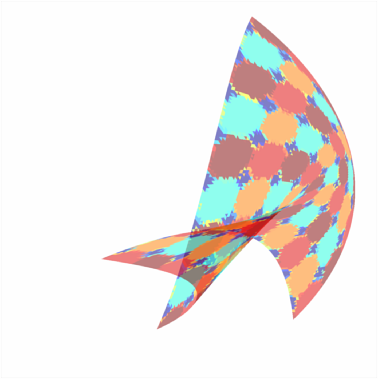
\includegraphics[width=0.33\columnwidth,clip=true,trim=10mm 10mm 1mm 1mm]{\topologyfiguresdir/manifold} &
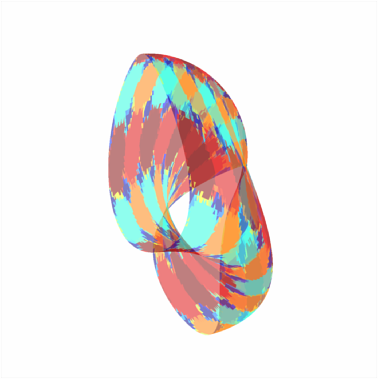
\includegraphics[width=0.33\columnwidth,clip=true,trim=10mm 10mm 10mm 10mm]{\topologyfiguresdir/cylinder} &
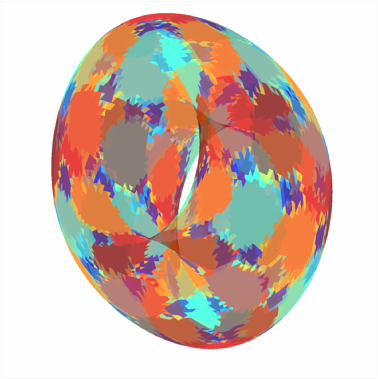
\includegraphics[width=0.33\columnwidth,clip=true,trim=1mm 1mm 1mm 1mm]{\topologyfiguresdir/torus} \\
\end{tabular}
\caption[Generating 2D manifolds with different topological structures]{
Generating 2D manifolds with different topologies.
By enforcing that the functions mapping from $\mathbb{R}^2$ to $\mathbb{R}^3$ obey certain symmetries, the surfaces created have corresponding topologies, ignoring self-intersections.
}
\label{fig:gen_surf}
\end{figure}

\Cref{fig:gen_surf} shows 2D meshes warped into 3D by functions drawn from \gp{} priors with various kernels, giving rise to a different topologies.
%
Higher-dimensional analogues of these shapes can be constructed by increasing the latent dimension and including corresponding terms in the kernel.
For example, an $N$-dimensional latent space using kernel $\kPer_1 \kerntimes \kPer_2 \kerntimes \ldots \kerntimes \kPer_N$ will give rise to a prior on manifolds having the topology of $N$-dimensional toruses, ignoring self-intersections.

This construction is similar in spirit to the \gp{} latent variable model (\gplvm{}) of \citet{lawrence2005probabilistic}, which learns a latent embedding of the data into a low-dimensional space, using a \gp{} prior on the mapping from the latent space to the observed space.



\subsection{M\"{o}bius strips}

%A prior on functions on M\"{o}bius strips can be constructed by enforcing the symmetries:

%
\begin{figure}
\begin{tabular}[t]{ccc}
%\begin{columns}
\centering
Draw from \gp{} with kernel: &  &  \\
%$( \Per_1 \times \Per_2 )$ and $f(x,y) = f(y,x)$ & generated parametrically\\
$\begin{array}{l@{}l@{}}
&            \Per(x_1, x_1') \kerntimes \Per(x_2, x_2') \\
 \kernplus & \Per(x_1, x_2') \kerntimes \Per(x_2, x_1')
\end{array}$
& $\begin{array}{c} \textnormal{ M\"{o}bius strip drawn from}  \\ \textnormal{$\mathbb{R}^2 \to \mathbb{R}^3$ \gp{} prior}  \end{array}$
 & $\begin{array}{c} \textnormal{Sudanese M\"{o}bius strip}  \\ \textnormal{generated parametrically}  \end{array}$\\
%$ + \Per(x_1, x_2') \times \Per(x_2, x_1')$ & \\
%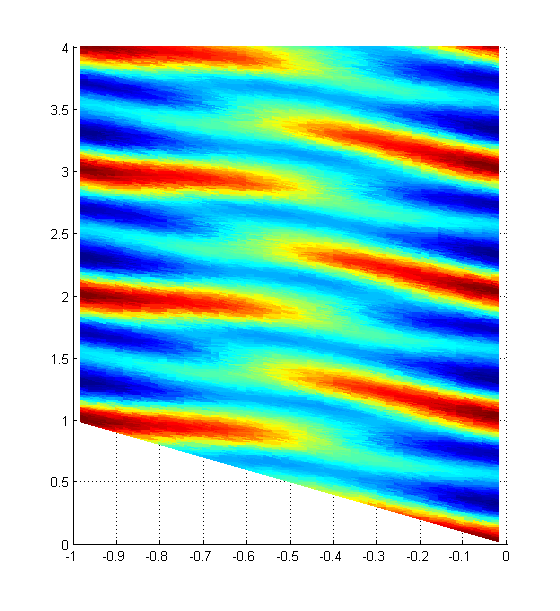
\includegraphics[width=0.45\columnwidth, height=0.45\columnwidth, clip=true,trim=2cm 2cm 2cm 1cm]{\topologyfiguresdir/mobius_regression} \\
\null\hspace{-5mm}\raisebox{2.75cm}{
\begin{tabular}{cc}
\raisebox{1.65cm}{$x_2$\hspace{-1.5mm}} &
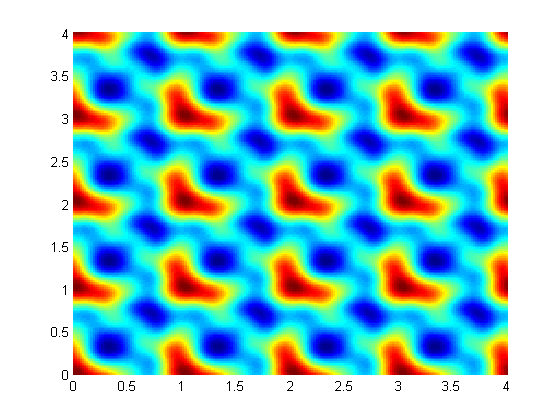
\includegraphics[width=0.235\columnwidth, height=0.235\columnwidth, clip=true,trim=3cm 2cm 2cm 2cm]{\topologyfiguresdir/mobius_field} \\
 & $x_1$ \\[-3em]
\end{tabular}}
& 
\raisebox{0.3cm}{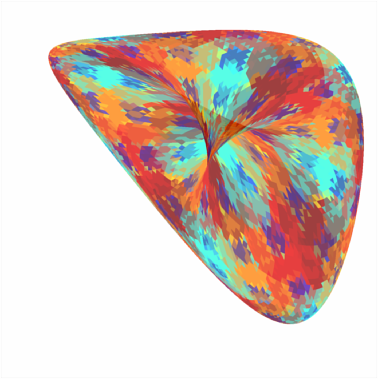
\includegraphics[width=0.3\columnwidth,clip=true,trim=1cm 1.3cm 1mm 1mm]{\topologyfiguresdir/mobius}} &
\raisebox{1cm}{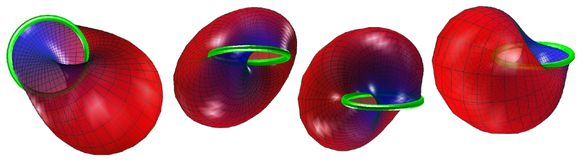
\includegraphics[width=0.25\columnwidth,clip=true,trim=0cm 0cm 14.6cm 0cm]{\topologyfiguresdir/sudanese-wikipedia}} \\[-0.5em]
\end{tabular}
\caption[Generating M\"{o}bius strips]{Generating M\"{o}bius strips.
\emph{Left:} A function drawn from a \sgp{} prior obeying the symmetries given by \cref{eq:mobius_symmetry_x,eq:mobius_symmetry_y,eq:mobius_symmetry_xy}.
\emph{Center:} Simply-connected surfaces mapped from $\mathbb{R}^2$ to $\mathbb{R}^3$ by functions obeying those symmetries have a topology corresponding to a M\"{o}bius strip.
Surfaces generated this way do not have the familiar shape of a flat surface connected to itself with a half-twist.
Instead, they tend to look like \emph{Sudanese} M\"{o}bius strips \citep{sudanese1984}, whose edge has a circular shape.
\emph{Right:} A Sudanese projection of a M\"{o}bius strip.
Image adapted from \citet{sudanesepict}.
}
\label{fig:mobius}
\end{figure}
%

A space having the topology of a M\"{o}bius strip can be constructed by enforcing invariance to the following operations~\citep[chapter 7]{reid2005geometry}:
%A function defined on a M\"{o}bius strips can be constructed by enforcing the symmetries~\citep[chapter 7]{reid2005geometry}:
%
%\begin{align}
%f(x_1, x_2) & = f( x_1 + \tau, x_2) \qquad \textnormal{(periodic in $x_1$)} \label%{eq:mobius_symmetry_x} \\
%f(x_1, x_2) & = f( x_1, x_2 + \tau) \qquad \textnormal{(periodic in $x_2$)} \label%{eq:mobius_symmetry_y} \\
%f(x_1, x_2) & = f( x_2, x_1)  \quad \,\,\,\; \qquad \textnormal{(symmetric about $x_1 = x_2$)}
%\label{eq:mobius_symmetry_xy}
%\end{align}
\begin{align}
g_{p_1}([x_1, x_2]) & = [ x_1 + \tau, x_2] \qquad \textnormal{(periodic in $x_1$)} \label{eq:mobius_symmetry_x} \\
g_{p_2}([x_1, x_2]) & = [ x_1, x_2 + \tau] \qquad \textnormal{(periodic in $x_2$)} \label{eq:mobius_symmetry_y} \\
g_s([x_1, x_2]) & = [ x_2, x_1]  \quad \,\,\,\; \qquad \textnormal{(symmetric about $x_1 = x_2$)}
\label{eq:mobius_symmetry_xy}
\end{align}
%
\Cref{sec:expressing-symmetries} already showed how to build \gp{} priors invariant to each of these types of transformations.
We'll call a kernel which enforces these symmetries a \emph{M\"{o}bius kernel}.
An example of such a kernel is:
%
\begin{align}
k(x_1, x_2, x_1', x_2') = 
\Per(x_1, x_1') \kerntimes \Per(x_2, x_2') \kernplus
\Per(x_1, x_2') \kerntimes \Per(x_2, x_1')
\end{align}
%
Moving along the diagonal $x_1 = x_2$ of a function drawn from the corresponding \gp{} prior is equivalent to moving along the edge of a notional M\"{o}bius strip which has had that function mapped on to its surface.
\Cref{fig:mobius}(left) shows an example of a function drawn from such a prior.
\Cref{fig:mobius}(center) shows an example of a 2D mesh mapped to 3D by functions drawn from such a prior.
This surface doesn't resemble the typical representation of a M\"{o}bius strip,
%, because the edge of the M\"{o}bius strip is in roughly circular shape, as opposed to the double-loop that one obtains by gluing a strip of paper with a single twist.
but instead resembles an embedding known as the Sudanese M\"{o}bius strip \citep{sudanese1984}, shown in \cref{fig:mobius}(right).

%Another classic example of a function living on a Mobius strip is the auditory quality of 2-note intervals.  The harmony of a pair of notes is periodic (over octaves) for each note, and the 



\section{Kernels on categorical variables}

%Kernels can be defined over all types of data structures: Text, images, matrices, and even kernels . Coming up with a kernel on a new type of data used to be an easy way to get a NIPS paper.

%\subsection{}

%There is a simple way to do \gp{} regression over categorical variables:
Categorical variables are variables which can take values only from a discrete, unordered set, such as $\{\texttt{blue}, \texttt{green}, \texttt{red}\}$.
A simple way to construct a kernel over categorical variables is to represent that variable by a set of binary variables, using a one-of-k encoding.
For example, if $\vx$ can take one of four values, $x \in \{ \texttt{A}, \texttt{B}, \texttt{C}, \texttt{D}\}$, then a one-of-k encoding of $x$ will correspond to four binary inputs, and $\oneofk(\texttt{C}) = [0, 0, 1, 0]$.
Given a one-of-k encoding, we can place any multi-dimensional kernel on that space, such as the \seard{}:
%
\begin{align}
k_{\textnormal{categorical}}( x, x') = \seard( \oneofk(x), \oneofk(x') )
\end{align}
%
Short lengthscales on any particular dimension of the $\seard$ kernel indicate that the function value corresponding to that category is uncorrelated with the others.
More flexible parameterizations are also possible~\citep{pinheiro1996unconstrained}.
%A more flexible parameterization suggested by 
%\citet{swersky2013categorical}
%Kevin Swersky (personal communication) allows complete flexibility about which pairs of categories are similar to one another, replacing the $\seard$ kernel with a fully-parameterized kernel, $\sefull$:
%
%\begin{align}
%\sefull( \vx, \vx') = \sigma^2_f \exp \left( -\frac{1}{2} \vx\tra \vL \vx' \right)
%\end{align}
%
%where $\vL$ is a symmetric matrix, individually parameterizing the covariance between each pair of function values of categories.



%Then, simply put a product of kernels on those dimensions.
%This is the same as putting one SE ARD kernel on all of them.
%Learning the lengthscale on each dimension of the $\kSE$ kernel will now encode how similar the value of the different categories are to one another.
%The lengthscale hyperparameter will now encode whether, when that coding is active, the rest of the function changes.
%If you notice that the estimated lengthscales for your categorical variables is short, your model is saying that it's not sharing any information between data of different categories. 


\section{Multiple outputs}

Any \gp{} prior can easily be extended to the model multiple outputs: ${f_1(\vx), f_2(\vx), \dots, f_T(\vx)}$.
This can be done by building a model of a single-output function which has had an extra input added that denotes the index of the output: $f_i(\vx) = f(\vx, i)$.
This can be done by extending the original kernel $k(\vx, \vx')$ to have an extra discrete input dimension: $k(\vx, i, \vx', i')$.

A simple and flexible construction of such a kernel multiplies the original kernel $k(\vx, \vx')$ with a categorical kernel on the output index~\citep{bonilla2007multi}:
%
\begin{align}
k(\vx, i, \vx', i') = k_{\vx}(\vx, \vx') \kerntimes k_i(i,i')
\end{align}






\iffalse

\section{Worked example: Building a structured kernel for a time-series}

%\subsection{Modeling multiple periodicities}

\begin{figure}[h]
\begin{tabular}{ccc}
Long-term trend & Weekly periodicity &Yearly periodicity \\
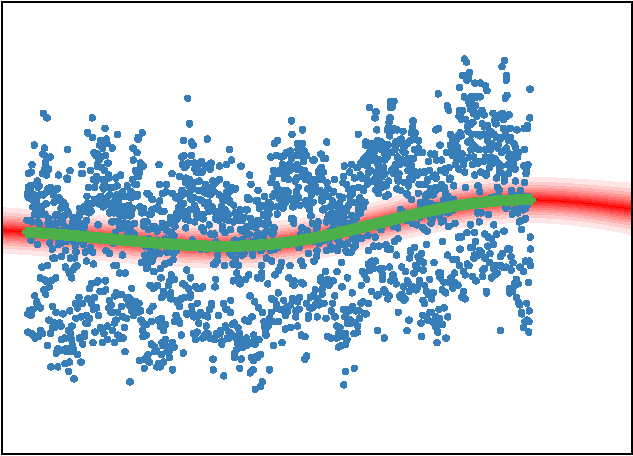
\includegraphics[width=0.31\columnwidth]{\examplefigsdir/births-component-1} &
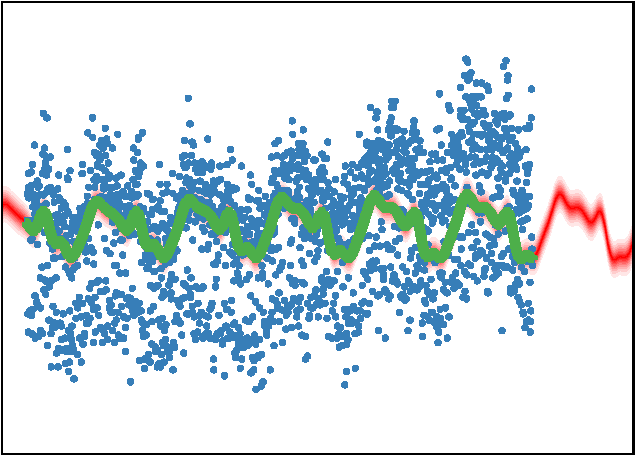
\includegraphics[width=0.31\columnwidth]{\examplefigsdir/births-component-3} & 
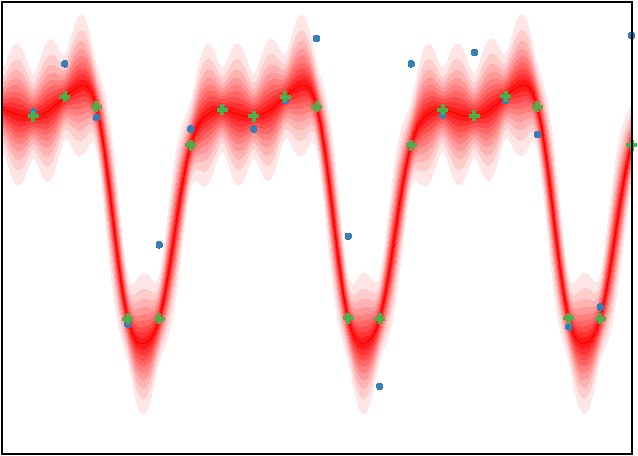
\includegraphics[width=0.31\columnwidth]{\examplefigsdir/births-component-2-zoom} 
\end{tabular}
\caption[Composite model of births data]{A composite \gp{} model of births data. (blue)}
\label{fig:quebec-decomp}
\end{figure}





\iffalse
\begin{figure}
\renewcommand{\tabcolsep}{1mm}
\def \incpic#1{\includegraphics[width=0.200\columnwidth]{../figures/worked-example/births-#1}}
\begin{tabular}{*{5}{c}}
 & {Long-term} & {Weekly} & {Yearly} & {Short-term} \\ 
 \rotatebox{90}{{Long-term}} & \incpic{Long-term-Long-term} & \incpic{Long-term-Weekly} & \incpic{Long-term-Yearly} & \incpic{Long-term-Short-term} \\ 
 \rotatebox{90}{{Weekly}} & \incpic{Weekly-Long-term} & \incpic{Weekly-Weekly} & \incpic{Weekly-Yearly} & \incpic{Weekly-Short-term} \\ 
 \rotatebox{90}{{Yearly}} & \incpic{Yearly-Long-term} & \incpic{Yearly-Weekly} & \incpic{Yearly-Yearly} & \incpic{Yearly-Short-term} \\ 
 \rotatebox{90}{{Short-term}} & \incpic{Short-term-Long-term} & \incpic{Short-term-Weekly} & \incpic{Short-term-Yearly} & \incpic{Short-term-Short-term} \\ 
 \end{tabular}
\caption[Two-way interactions in births data]{Two-way interactions in births data}
\label{fig:quebec-decomp}
\end{figure}
\fi
%\subsection{Incoportating discrete covariates}

%\subsection{Breaking down the predictions, examining different parts of the model}
\fi





\section{Building a kernel in practice}

%\subsection{Learning Kernel Parameters}

This chapter outlined ways to choose the parametric form of a kernel in order to express different sorts of structure.
Once the parametric form has been chosen, one still needs to choose, or integrate over, the kernel parameters.
%Fortunately, typical kernels only have $\mathcal{O}(D)$ parameters, meaning that if $N$ is reasonably large, these parameters can be estimated by maximum marginal likelihood.
If the kernel relatively few parameters, these parameters can be estimated by maximum marginal likelihood, using gradient-based optimizers.
The kernel parameters estimated in \cref{sec:additivity-extrapolation,sec:concrete} were optimized using the \GPML{} toolbox~\citep{GPML}, available at \\\url{http://www.gaussianprocess.org/gpml/code}.

%\subsection{Choosing the Kernel Form}
%The marginal likelihood of a model is useful for choosing among parameters.
%The marginal likelihood can also be used to selecting which type of kernel to use.
% the form of the kernel.
%For example, we might not know whether a particular structure or symmetry is present in the function we are trying to model.
%Again, the fact that we can compare marginal likelihoods in \gp{}s means that we can 
%Because \gp{}s let us build models both with and without certain symmetries, 
%By building kernels with and without such structure, we can compute the marginal likelihoods of the corresponding \gp{} models.
%The quantities represent the relative amount of evidence that the data provide for each of these possibilities, providing the assumptions of the model are correct.
%To do so, we simple need to compare the marginal likelihood of the data
%We demonstrate that marginal likeihood an be used to automatically search over such structures.

A systematic search over kernel parameters is necessary when appropriate parameters are not known.
Similarly, sometimes appropriate kernel structure is hard to guess.
The next chapter will show how to perform an automatic search not just over kernel parameters, but also over an open-ended space of kernel expressions.

\subsubsection{Source code}
Source code to produce all figures and examples in this chapter is available at \\\url{http://www.github.com/duvenaud/phd-thesis}.

%\section{Conclusion}

%We've seen that kernels are a flexible and powerful language for building models of different types of functions.
%However, for a given problem, it can difficult to specify an appropriate kernel, even after looking at the data.
%A better procedure would be to compare the predictive performance, or marginal likelihood, of a few different kernels.
%However, it might be difficult to enumerate all plausible kernels, and tedious to search over them.
%In fact, choosing the kernel can be considered one of the main difficulties in doing inference.

%Analogously, we usually don't expect to simply guess the best value of some parameter.
%Rather, we specify a search space and an objective, and ask the computer to the search this space for us. 



\outbpdocument{
\bibliographystyle{plainnat}
\bibliography{references.bib}
}



\iffalse


\subsection{Example: Computing Molecular Energies}

\begin{figure}
\begin{center}
\begin{tabular}{cc}
Function on M\"{o}bius strip & \\
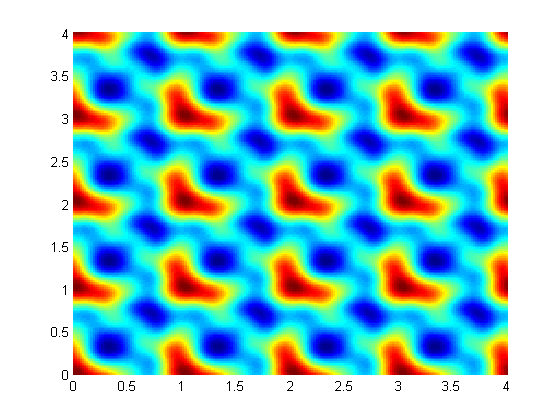
\includegraphics[width=0.3\columnwidth, height=0.3\columnwidth, clip=true,trim=3cm 2cm 2cm 2cm]{\topologyfiguresdir/mobius_field} & 
  \begin{tikzpicture}

%\pgfmathsetmacro{\r}{3cm}
%\pgfmathsetmacro{\ho}{70}
%\pgfmathsetmacro{\ht}{30}
\newcommand{\radius}{3}
\newcommand{\hone}{120}
\newcommand{\htwo}{70}
\newcommand{\hthree}{30}

	\coordinate (O) at (0, 0);
	\coordinate (left) at ({\radius*cos(\hone)}, {\radius*sin(\hone)});
	\coordinate (right) at ({\radius*cos(\htwo)}, {\radius*sin(\htwo)});
	\coordinate (zero) at ({\radius*cos(\hthree)}, {\radius*sin(\hthree)});

	\draw[fill] (left) circle (2pt);
	\draw (left) node[below, left] {H};
	
	\draw[fill] (right) circle (2pt);
	\draw (right) node[right] {H};

	\draw[fill] (zero) circle (2pt);
	\draw (zero) node[right] {H};

	\draw[fill] (O) circle (3pt);
	\draw (O) node[below] {C};

	\draw (left) -- (O);
	\draw (right) -- (O);
	\draw (zero) -- (O);

	\begin{scope}
	\path[clip] (O) -- (right) -- (zero);
	\fill[red, opacity=0.5, draw=black] (O) circle (2);
	\node at ($(O)+(50:1.6)$) {$\theta_1$};	
	\end{scope}
	
	\begin{scope}
	\path[clip] (O) -- (left) -- (right);
	\fill[green, opacity=0.5, draw=black] (O) circle (1.8);
	\node at ($(O)+(90:1.4)$) {$\theta_2$};	
	\end{scope}	
  \end{tikzpicture}
\end{tabular}
\end{center}
\caption[The energy of a molecular configuration obeys the same symmetries as a M\"{o}bius strip]{An example of a function expressing the same symmetries as a M\"{o}bius strip in two of its arguments.  The energy of a molecular configuration $f(\theta_1, \theta_2)$ depends only on the relative angles between atoms, and because each atom is indistinguishable, is invariant to permuting the atoms. }
\label{fig:molecule}
\end{figure}

Figure \ref{fig:molecule} gives one example of a function which obeys the same symmetries as a M\"{o}bius strip, in some subsets of its arguments.

\fi
